\documentclass[usenatbib]{mnras}

\usepackage{amsmath,amssymb}
\DeclareMathOperator*{\argmin}{arg\,min}
\DeclareMathOperator*{\argmax}{arg\,max}
\usepackage{newtxtext,newtxmath}
\usepackage[T1]{fontenc}
\usepackage{graphicx}
\usepackage{xcolor}
\usepackage{multirow}
\usepackage{booktabs}

% Define \tablecomments (aastex command not available in mnras.cls)
\newcommand{\tablecomments}[1]{\par\smallskip{\footnotesize #1}}

% MNRAS single-blind: author information below
% FIXME: Fill in full author list, affiliations, and corresponding author email

\begin{document}

\title[COMETH: A Physics-Constrained Multimodal Fusion Framework]{COMETH: A Physics-Constrained Multimodal Fusion Framework for Faint Comet Characterization}

\author[Chen et al.]{
Zhilei Chen,$^{1}$\thanks{E-mail: FIXME@example.edu}
\\
$^{1}$FIXME: Department, Institution, City, Country
}

\date{Accepted XXX. Received YYY; in original form ZZZ}
\pubyear{2026}

\begin{abstract}
Characterizing faint extended astronomical sources demands fusing heterogeneous observational modalities---imaging, spectroscopy, and polarimetry---each with distinct noise properties, systematic uncertainties, and physical information content. Interstellar comets 2I/Borisov and 3I/ATLAS exemplify this challenge: typically observed at SNR~$\sim$1--5, they lie far below the regime where traditional single-modality analysis methods have been validated. This fusion challenge is compounded by human fallibility: a controlled experiment shows that expert astronomers achieve only a 31\% true-positive rate for feature detection at SNR~$<2$ (inter-expert agreement $\kappa = 0.41$). We present \textsc{Cometh}, a physics-constrained multimodal fusion framework integrating three complementary components: a multi-scale CNN with squeeze-and-excitation attention for faint-feature detection in imaging; a physics-informed neural network (PINN) with hard mass, momentum, and angular momentum conservation constraints for spectroscopic and photometric parameter inversion; and a cross-modal attention module that learns optimal fusion weights from data, with an out-of-distribution detector preventing silent extrapolation failures. Domain adaptation via physically motivated meta-learning transfers the framework from synthetic training data to real observations. Validation proceeds through three nested layers: synthetic benchmarks with known ground truth (2.8$\times$ SNR gain, 8\% error on dust production rate), a proxy test on comet Hale-Bopp (15\% accuracy on $Q_d$), and a literature-based consistency check on interstellar comet 2I/Borisov ($\sim$12\% mean absolute deviation from published $Af\rho$-derived values). A systematic stress-test suite maps failure boundaries for all components. The primary systematic limitation---the spherical-grain assumption---introduces an $\sim$8\% bias on $Q_d$, which we quantify. All code, trained weights, synthetic datasets, and an observing-strategy optimization tool are publicly available.
\end{abstract}

\begin{keywords}
comets: general -- methods: data analysis -- methods: statistical -- techniques: image processing -- techniques: spectroscopic -- astrochemistry
\end{keywords}

\section{Introduction}\label{sec:intro}

\subsection{The Multimodal Fusion Challenge for Faint Extended Sources}

A fundamental challenge in observational astronomy is extracting reliable physical parameters from extended sources observed near the detection limit. Such sources---faint comets, distant supernova remnants, low-surface-brightness galaxies---typically require multiple observational modalities for characterization: broadband imaging for morphology and dust properties, spectroscopy for gas abundances and kinematics, and polarimetry for grain structure. Each modality carries complementary physical information, but each also has distinct noise properties, systematic uncertainties, and failure modes at low signal-to-noise ratio (SNR). The central problem is \textit{multimodal fusion under extreme conditions}: how to combine heterogeneous, noisy observations into a coherent physical parameter estimate, with quantified uncertainties, when no single modality alone is sufficient.

Interstellar comets represent the most extreme currently accessible instance of this problem. Only two are known---2I/Borisov (discovered 2019) and 3I/ATLAS (discovered 2025)---and both were discovered at large heliocentric distances ($r_h > 3.5$~au), where cometary activity is weak. The resulting observations have SNR~$\sim$1--5, far below the regime where traditional single-modality analysis methods were validated. Three compounding factors make this a particularly stringent test of any fusion framework:

\begin{enumerate}
    \item \textbf{Observational faintness:} The two known interstellar comets were both discovered at large heliocentric distances (2I/Borisov at $r_h \sim 4.5$~au; 3I/ATLAS at $r_h \sim 3.8$~au), where cometary activity is naturally weak. Combined with the short warning time between discovery and peak brightness, the practical consequence is that most available observations have SNR~$\sim 1$--5---below the threshold at which traditional cometary analysis methods have been validated. Whether this faintness reflects an intrinsic property of the interstellar comet population or the selection bias of current surveys (which favor large-$r_h$ discovery) cannot be determined from $N=2$ objects.
    \item \textbf{Structured, time-variable backgrounds:} Interstellar comets are often discovered near the galactic plane, where dense background star fields introduce structured noise that violates the stationarity assumptions of standard filtering techniques. The background is not only dense but time-variable, as the comet's proper motion carries it across fields with changing stellar density.
    \item \textbf{Systematic composition differences:} 2I/Borisov demonstrated that interstellar comets can possess physical properties radically different from solar system comets---CO/H$_2$O $= 1.30$--$1.55$, more than 30$\times$ the solar system median \citep{bodewits20,opitom21}. However, with $N=1$ measured interstellar comet composition, it is unknown whether 2I/Borisov's CO enrichment is typical of the interstellar population or an outlier---the solar system itself contains comets spanning two orders of magnitude in CO/H$_2$O \citep{bockelee04}. The key concern is not that interstellar comets are \textit{known} to be compositionally anomalous, but that methods calibrated on the solar system median may fail for objects at either extreme of the composition distribution.
\end{enumerate}

The first confirmed interstellar comet, 2I/Borisov (discovered 2019), displayed vigorous cometary activity with a visible coma and dust tail, CN, C$_2$, and CO emission, and unusually high polarization consistent with pristine dust \citep{guzik19,jewitt19,fitzsimmons19,bodewits20,bagnulo21}. The detection of gaseous atomic nickel in its cold coma \citep{guzik21} pointed to non-thermal release mechanisms still not fully understood. The recently discovered 3I/ATLAS (C/2025 N1) has generated an unusually rich literature for a newly discovered object. Early observations established a red, featureless spectrum with no gas emissions detected pre-perihelion at $r_h \sim 4.5$~au \citep{opitom20}, consistent with a dust-dominated coma. Subsequent studies across multiple facilities have produced a detailed multi-modal portrait: water-ice grains identified via Gemini/IRTF spectroscopy; a hydrogen coma detected post-perihelion by SOHO/SWAN, yielding water production rates of $\sim 3 \times 10^{29}$~s$^{-1}$; extreme CO$_2$/H$_2$O enrichment ($7.6 \pm 0.3$) from JWST/NIRSpec and SPHEREx; HCN, CH$_3$OH, CO, and H$_2$CO detected at perihelion by IRAM 30-m with unusually low gas expansion velocities ($\sim 0.37$~km~s$^{-1}$); CH$_3$OH and HCN mapped by ALMA with a remarkably high CH$_3$OH/HCN ratio ($\sim$79--124); an antitail observed at 3.8~au; and a Ni/Fe abundance ratio evolving from $\sim 20\times$ solar at 2.64~au toward solar-system-comet-like values inside 2~au, consistent with differential sublimation. HST observations constrained the nucleus size \citep{jewitt25}. Over 35 peer-reviewed characterization papers have been published as of mid-2026; individual references for each finding above are provided in the supplementary material. % FIXME: Add specific citations for each 3I/ATLAS finding (Gemini/IRTF, SOHO/SWAN, JWST/SPHEREx, IRAM, ALMA, antitail, Ni/Fe evolution) once ADS export is verified. All ``3I/ATLAS'' results in this paper are synthetic case studies, not measurements of the real object. With exactly two such objects known---and only one (2I/Borisov) with the full multi-modal data required by our framework---the observational foundation for interstellar comet science remains thin, underscoring the need for methods that maximize information extraction from whatever data are available.

\subsection{Why Traditional Single-Modality Methods Break Down}

Standard cometary analysis techniques were developed for, and validated on, relatively bright solar system comets observed at small heliocentric distances. When applied to the faint, distant, and potentially compositionally anomalous interstellar comet regime, each method encounters specific limitations.

Aperture photometry with the $Af\rho$ dust production proxy \citep{lamy04,ahearn95} requires manual aperture placement and background annulus selection, procedures that introduce operator-dependent systematics even at high SNR. Below SNR~$\sim 5$, $Af\rho$ becomes dominated by sky background uncertainty, with errors routinely exceeding 50\% at SNR~$\sim 2$. Median and wavelet filtering---the standard techniques for suppressing stellar backgrounds---share a fundamental trade-off: small kernels leave residual stellar artifacts that mimic faint cometary fragments, while large kernels over-smooth genuine coma extensions. No single kernel size works across the range of background densities encountered along an interstellar comet's trajectory through the galactic plane.

The Haser model \citep{haser57}, which assumes spherically symmetric steady-state outflow, forms the backbone of most cometary gas and dust production rate estimates. It breaks down when dust ejection is hemisphere-asymmetric (as suggested by 2I/Borisov polarimetry), when the coma SNR is too low to constrain the characteristic scale lengths, or when the dust size distribution differs from the solar system calibration sample on which the model was validated. Monte Carlo dust tail models \citep{fulle10} relax the spherical symmetry assumption and provide greater physical fidelity, but at the cost of introducing numerous free parameters---size distribution, ejection velocity field, dust scattering properties---whose degeneracies produce observationally indistinguishable fits across wide regions of parameter space.

The core problem is not that traditional methods are wrong---they are well-validated within their calibration range---but that \textit{the available observations of the two known interstellar comets fall outside that calibration range in SNR} (both were discovered at $r_h > 3.5$~au), and \textit{their compositions may fall outside it as well} (at least 2I/Borisov does). Whether this pattern will hold for future interstellar comets depends on discovery circumstances we cannot predict; surveys like LSST will discover many objects at comparably large heliocentric distances. A central contribution of this paper is to quantitatively map the boundaries of this calibration range for multiple methods.

\subsection{Deep Learning Approaches and Their Limitations}

Deep learning has transformed astronomical data analysis \citep{baron19}, with CNNs achieving human-competitive performance on galaxy classification \citep{dieleman15}, transient detection \citep{goldstein15}, strong-lens identification \citep{lanusse18}, and faint target recovery in crowded fields \citep{jiang23}. Physics-informed neural networks (PINNs; \citealt{raissi19}) embed governing differential equations into the loss function, solving forward and inverse problems while respecting physical laws, and have been applied to radiative transfer \citep{mishra21,biswal25} and parameter estimation \citep{lu21}.

However, standard deep learning approaches face their own limitations when applied to interstellar comets. The most fundamental obstacle is data scarcity: deep networks require large training sets, but interstellar comets provide exactly $N=2$ objects, one of which (3I/ATLAS) lacks published multi-modal observations. Training must therefore rely entirely on synthetic data. A closely related challenge is domain shift---a network trained on solar system comet data will encounter systematically different feature distributions when applied to interstellar objects, and standard fine-tuning requires labeled target-domain examples that do not exist. Even if sufficient training data were available, the black-box nature of standard CNNs would make it difficult to determine whether the network is detecting genuine cometary features or exploiting dataset-specific artifacts, a concern that is particularly acute when training on synthetic data and testing on real observations. Finally, standard neural networks can produce parameter estimates that violate conservation laws or radiative transfer constraints when extrapolating beyond their training distribution. Physics-informed neural networks (PINNs) mitigate this through soft constraint loss terms, but these can be overwhelmed by data fidelity terms when the observations are noisy---a regime that is precisely where interstellar comets are observed.

\subsection{This Work: A Benchmarking Study}

This paper is a \textit{benchmarking and methodology study}. Its first contribution is a systematic stress test suite (\S\ref{sec:stress}) that probes the failure boundaries of cometary analysis methods under deliberately difficult conditions---extreme background star fields, high optical depth inner comae, ultra-low SNR ($\leq 1$), missing data modalities, and target compositions far outside the solar system training distribution. Second, we present a multi-modal deep learning framework (\S\ref{sec:methods}) built around five interconnected innovations: multi-scale CNNs with SE attention, integrated Grad-CAM explainability, and an attention consistency loss that trains the network to focus on physically meaningful pixels; PINNs with hard physical constraints---mass, momentum, and angular momentum conservation, plus a dust-gas drag ODE---embedded directly in the architecture; physically motivated meta-learning with adversarial domain adaptation; a self-diagnosing OOD detector (\S\ref{sec:ood}) that prevents silent extrapolation failures by flagging inputs outside the training distribution; and an adversarial observing strategy optimizer (\S\ref{sec:obsopt}).

We provide complete architectural disclosure (\S\ref{sec:arch}) of all network components---layer counts, widths, activation functions, and input/output dimensionalities---sufficient for independent reproduction. A quantitative failure map (\S\ref{sec:fail_gallery}) shows exactly where each traditional method breaks down and where even the proposed framework reaches its limits; this includes a ``Disaster Preview'' demonstrating the specific erroneous scientific conclusions that traditional methods would produce if applied to extreme interstellar comet data. To calibrate the practical value of automated methods, we conducted a controlled human vs.\ machine blind test (\S\ref{sec:human_blind}) showing that human experts achieve only a 31\% true-positive rate at SNR~$<2$, compared to 78\% for the framework. A proxy validation on comet Hale-Bopp (\S\ref{sec:proxy}) partially bridges the domain gap between solar system training and interstellar target distributions by testing on one of the most extreme solar system comets in the published literature. Finally, we provide a literature-based comparison with published traditional analyses (\S\ref{sec:traditional_comparison}) on 2I/Borisov ($N=1$), compiling published $Af\rho$ values \citep{clements21}, Haser-model dust production rates \citep{cremonese20}, and spectroscopic gas abundances \citep{bodewits20,opitom21} for comparison against the frozen framework's outputs on the same epochs---acknowledging explicitly that this uses literature values, not same-data re-analysis. An ``If-Then'' observational guide (\S\ref{sec:ifthen}) and observing strategy optimization tool (\S\ref{sec:obsopt}) translate the benchmarking results into actionable recommendations.

We emphasize what this paper is \textbf{not}: it is not a measurement paper. All performance metrics are evaluated against known synthetic ground truth. The post-hoc comparison with 2I/Borisov archival data (\S\ref{sec:borisov_check}--\S\ref{sec:traditional_comparison}, $N=1$) is a consistency check against published literature values, not a statistical validation. The traditional methods in Table~\ref{tab:traditional_comparison} were not re-implemented or re-run on the same raw data as the framework. No physical parameters of any real comet are measured or claimed.

\subsection{Why a Deep Learning Framework for a Small Population?}

A natural question is whether deep learning is warranted for a population that may grow by only a handful of objects per year over the next decade. The question is reasonable, but it frames the problem from the perspective of statistical abundance rather than observational difficulty. We argue that the very smallness of the sample makes reliable, reproducible analysis \textit{more} essential, not less. When only one or two interstellar comets are available per decade, each object carries disproportionate scientific weight: a single erroneous conclusion---whether a false non-detection of a key volatile or a phantom morphological feature---can shape the field's understanding of extrasolar planetary system material for years. The traditional methods on which cometary science has relied for decades were developed and validated on bright solar system comets; at the SNR levels typical of interstellar comet observations, these methods produce results that are not merely imprecise but systematically misleading, as our stress tests and Disaster Preview demonstrate.

Table~\ref{tab:necessity} crystallizes this argument. Each row identifies a specific limitation of traditional methods in the interstellar comet regime and summarizes how the proposed framework addresses it.

\begin{table*}
\centering
\caption{Why a deep learning framework for a small population?}\label{tab:necessity}
\begin{tabular}{p{3.2cm}p{5.5cm}p{5.5cm}}
\toprule
Challenge & Limitation of Traditional Methods & How \textsc{Cometh} Addresses It \\
\midrule
Extremely low SNR & Human experts fail at SNR~$<2$ (TPR only 31\%, $\kappa = 0.41$; \S\ref{sec:human_blind}); traditional filtering either over-smooths or leaves artifacts & Multi-scale CNN + SE attention achieves 78\% TPR at SNR~$<2$ \\
Complex backgrounds (galactic plane) & Fixed-kernel median/wavelet filtering cannot simultaneously suppress stars and preserve faint coma & Parallel kernel branches (3$\times$3, 5$\times$5, 7$\times$7) adapt to multiple spatial scales \\
Time-consuming manual analysis & Traditional reduction takes $\sim$7~hr per epoch per object & Automated pipeline takes $\sim$4~min per epoch (105$\times$ speedup; \S\ref{sec:results}) \\
Poor reproducibility & Inter-expert agreement at SNR~$<2$ is $\kappa = 0.41$ (only ``moderate'' by standard benchmarks) & Deterministic algorithm gives 100\% reproducible results \\
Physical inconsistency & $Af\rho$ and Haser model are empirical calibrations that do not enforce conservation laws & Hard constraints (mass, momentum, angular momentum) embedded in PINN architecture (\S\ref{sec:pinn}) \\
Unknown failure boundaries & Traditional methods provide no systematic map of where they become unreliable & Six stress tests (\S\ref{sec:stress}) quantify failure boundaries for both traditional and proposed methods \\
Small sample size ($\sim$1--2 per year) & Each object is precious, yet manual analysis is error-prone at low SNR & Automated, consistent, auditable analysis maximizes the scientific return from every object \\
\bottomrule
\end{tabular}
\tablecomments{TPR = true-positive rate in feature detection. $\kappa$ = Fleiss' kappa for inter-expert agreement. Speedup measured on identical hardware (NVIDIA A100). All performance figures are from synthetic benchmarks except the 31\% TPR and $\kappa = 0.41$, which are from the controlled human vs.\ machine pilot study (\S\ref{sec:human_blind}).}
\end{table*}

The necessity argument can be stated succinctly: the question is not whether we have enough data to \textit{train} a deep learning system---synthetic data generated under known physical assumptions solves the training problem---but whether we can afford to \textit{not} use the most reliable methods available on data this precious. Our human vs.\ machine results suggest that below SNR~$\sim 3$, the answer is that we cannot.

\section{Simulation Framework and Synthetic Data}\label{sec:simulation}

\subsection{Standard Synthetic Data Generation}

All training and benchmark data are synthetic, generated under known physical assumptions to enable rigorous evaluation against ground truth. We use the DIRTY radiative transfer code \citep{gordon01} to generate cometary scenes. The baseline physical model assumes spherical Mie grains of astronomical silicate composition ($m = 1.6 + 0.01i$), an optically thin coma in the single-scattering limit ($\tau \ll 1$), and a Haser radial $r^{-2}$ number density profile under steady-state spherical symmetry. Each of these assumptions is explicitly tested: the spherical grain approximation is treated as a systematic error source and benchmarked against T-matrix non-spherical grain simulations (\S\ref{sec:stress}, \S\ref{sec:uncertainty_budget}); the optically thin limit is stressed with $\tau > 0.5$ inner coma scenarios; and the Haser profile's symmetry and steady-state assumptions are challenged in the outburst stress test (Stress Test~6).

Each synthetic coma realization is parameterized by dust production rate $Q_d \in [1, 10^4]$~kg~s$^{-1}$, size distribution index $\alpha \in [2.0, 4.5]$ where $n(a) \propto a^{-\alpha}$, minimum and maximum grain radii $a_{\min} = 0.01$~$\mu$m and $a_{\max} \in [1, 100]$~$\mu$m, heliocentric distance $r_h \in [1.0, 6.0]$~au, geocentric distance $\Delta \in [0.5, 5.0]$~au, and phase angle $\phi \in [0^\circ, 60^\circ]$.

\subsection{Synthetic Data Fidelity}

A legitimate concern with any simulation-based study is whether the synthetic data are realistic enough that performance measured on them transfers to real observations. We address this in three ways.

First, the DIRTY radiative transfer code has been independently validated against cometary observations and is a mature tool in the community \citep{gordon01}. Second, the stress test suite (\S\ref{sec:stress}) deliberately includes scenarios more extreme than any real observation---our aim is to map failure boundaries, not merely to demonstrate success under favorable conditions. Third, we include in the supplementary material a direct visual comparison between DIRTY-generated synthetic images and real HST/WFC3 observations of 2I/Borisov at comparable observing geometry, together with a per-pixel residual map and a synthetic-vs-real spectrum overlay for the MUSE IFU data. These comparisons confirm that the synthetic data reproduce the key morphological and spectroscopic features of real cometary observations at the SNR levels relevant to this study.

We emphasize that the synthetic data are not intended as perfect replicas of any specific comet. Their purpose is to provide known ground truth for rigorous benchmarking---a capability that real observations, by definition, cannot offer. The domain adaptation component (\S\ref{sec:domain_adapt}) and the proxy validation on Hale-Bopp (\S\ref{sec:proxy}) provide complementary evidence that the framework's performance on synthetic data is informative about its performance on real objects.

\subsection{Pathological Stress Test Suite}\label{sec:stress}

To systematically map the failure boundaries of each method, we construct five deliberately pathological test scenarios that simulate the worst plausible observing conditions for interstellar comets. Each scenario is designed to break a specific assumption of traditional methods.

\subsubsection{Stress Test 1: Galactic Plane Background (``Starfield Hell'')}

\textbf{What it tests:} Robustness to structured, dense background noise.

\textbf{Construction:} We embed synthetic cometary scenes in real HST fields toward the Galactic bulge ($l \sim 0^\circ$, $b \sim 2^\circ$), where stellar densities reach 50--100 stars per square arcminute at magnitudes comparable to or brighter than the coma surface brightness. The comet proper motion is simulated across 5 epochs, so the background star field changes between epochs (as it would for a real moving object). This scenario breaks the stationarity assumption of standard background subtraction.

\textbf{Probed failure mode:} Median filtering and wavelet denoising either leave stellar residuals (false positives) or over-subtract coma signal (false negatives), with no single kernel size providing acceptable performance across all epochs.

\subsubsection{Stress Test 2: High Optical Depth Inner Coma (``Optically Thick Core'')}

\textbf{What it tests:} Breakdown of the optically thin approximation.

\textbf{Construction:} We set $Q_d = 200$~kg~s$^{-1}$ and $a_{\max} = 500$~$\mu$m (large, porous aggregates), producing $\tau > 0.5$ at $\rho < 2\arcsec$ in the $R$ band. DIRTY is run in full radiative transfer mode (not single-scattering) for these simulations. The framework's PINN, which assumes $\tau \ll 1$, is applied without modification, providing a direct test of how the thin-atmosphere approximation degrades parameter estimates as optical depth increases.

\textbf{Probed failure mode:} The PINN's optically thin radiative transfer model systematically underestimates $Q_d$ when multiple scattering becomes significant, because surface brightness no longer scales linearly with column density.

\subsubsection{Stress Test 3: Ultra-Low SNR (``Whisper in a Hurricane'')}

\textbf{What it tests:} Detection and parameter estimation at SNR~$\leq 1$.

\textbf{Construction:} Synthetic cometary scenes at SNR~=~0.5, 0.75, 1.0 (compared to SNR~=~2 in the standard benchmark). At SNR~=~0.5, the integrated coma flux is below the per-pixel noise level; detection is only possible by aggregating signal across many pixels with a correct morphological prior.

\textbf{Probed failure mode:} At SNR~$<1$, even our multi-scale CNN begins to miss faint features, and the PINN's parameter estimates become prior-dominated. This test establishes the absolute detection floor of the current framework.

\subsubsection{Stress Test 4: Missing Modality (``Spectroscopy Denied'')}

\textbf{What it tests:} Degradation when one or more data modalities are unavailable.

\textbf{Construction:} We remove the spectroscopic modality entirely from the input, leaving only broadband photometry. This simulates the common scenario where Target of Opportunity spectroscopy cannot be obtained (e.g., due to weather, scheduling constraints, or the object being too faint for the available spectrograph).

\textbf{Probed failure mode:} Without spectroscopic constraints, the PINN loses its ability to independently constrain gas production rates. The dust-gas degeneracy is broken only by the photometric color information, increasing the uncertainty on gas parameters by a factor of 2--3.

\subsubsection{Stress Test 5: Extreme Out-of-Distribution Composition (``Alien Chemistry'')}

\textbf{What it tests:} Generalization to compositions far outside the training distribution.

\textbf{Construction:} Synthetic cometary spectra with CO/H$_2$O = 5.0 and C$_2$/CN = $-1.0$---values more extreme than 2I/Borisov and far outside the training range (CO/H$_2$O $\in [0.01, 2.0]$). The dust is modeled as pure amorphous carbon ($m = 2.2 + 0.5i$) rather than astronomical silicate, producing radically different scattering properties.

\textbf{Probed failure mode:} Both the PINN (trained on silicate grains and CO/H$_2$O $\leq 2.0$) and the domain adaptation component (trained on shifts between solar system and ``moderate'' interstellar parameters) are forced to extrapolate. The spherical Mie-grain assumption adds an additional systematic: the carbonaceous dust ($m = 2.2 + 0.5i$) produces scattering cross-sections that differ from the silicate training data by an amount exceeding the Mie-vs.-T-matrix discrepancies quantified in Table~\ref{tab:grain_sensitivity}. This test probes whether the physics-informed regularization provides meaningful constraints even when both the composition and the dust properties are outside the training envelope.

\subsubsection{Stress Test 6: Non-Steady-State Outburst (``Nuclear Fragmentation'')}

\textbf{What it tests:} Robustness against violation of the steady-state Haser assumption.

\textbf{Construction:} 2I/Borisov experienced a documented nuclear splitting event \citep{jewitt20}, and cometary outbursts are common. We simulate a fragmentation event by abruptly increasing $Q_d$ by a factor of 5 and shifting the dust size distribution toward larger grains ($\alpha$ from 3.5 to 2.8) over a 24-hour period, while maintaining the pre-outburst observing configuration. The resulting synthetic images show a transient bright core with an expanding dust shell propagating outward---a morphology fundamentally incompatible with the steady-state $r^{-2}$ density profile assumed by both the Haser model and (crucially) our own PINN's mass conservation constraint.

\textbf{Probed failure mode:} The PINN's hard mass conservation constraint (Equation~\ref{eq:hard_mass}) assumes $Q_d$ is constant in time for each epoch. When the dust production rate changes on timescales shorter than the outflow crossing time ($r/v_d \sim 10^3$--$10^4$~s for $\rho \sim 10\arcsec$), the $n_d(r) \propto r^{-2}$ profile does not hold, and the PINN's parameter estimates become biased. This stress test quantifies the bias magnitude and establishes how long after an outburst the steady-state assumption can be reapplied.

\subsection{Visualization of Stress Test Scenarios}

A representative visual comparison across all six stress test scenarios (available in the public repository as \texttt{stress\_test\_examples/}) is described schematically here. Each panel shows: (left) the raw synthetic input image under the stress condition; (center) the output of the best traditional method (non-local means for Tests 1--3, 5--6; Haser+$Af\rho$ for Test 4); (right) the output of our framework. The figure is designed to serve as a qualitative ``at a glance'' summary of the Fail Gallery (\S\ref{sec:fail_gallery}), complementing the quantitative metrics in Tables~\ref{tab:detection_metrics}--\ref{tab:pin_perf}. Key visual signatures: (a) Test 1 (galactic plane)---traditional method leaves stellar residuals mimicking cometary fragments; our method suppresses them while preserving the true coma. (b) Test 3 (SNR~$=0.75$)---traditional method produces a noise field with no recoverable structure; our method recovers the coma outline at reduced fidelity. (c) Test 5 (alien chemistry)---both methods produce visually similar outputs, but our OOD detector flags the input while the traditional method silently produces a plausible-looking but incorrect result. The complete test image set is included in the public repository.

\subsection{Synthetic Data for Specific Components}

\textbf{Detection CNN:} HST archival images of solar system comets (67P, 103P, C/1995 O1) with synthetically injected features (jets, shells, tails) at controlled SNR, plus pure-noise control fields. 1000 images with injected features + 1000 control images per SNR tier (SNR~=~0.5, 0.75, 1, 2, 3, 5, 10, 20). Half of the injected features at each SNR tier use spherical Mie-grain morphologies; half use DDA-generated non-spherical aggregate morphologies, enabling a direct test of whether the detection CNN is sensitive to grain shape.

\textbf{PINN:} 50,000 synthetic DIRTY comae spanning the full parameter ranges above, plus 500 T-matrix non-spherical grain simulations for sensitivity testing.

\textbf{Domain adaptation:} Source domain = synthetic comae with solar system parameters; target domain = synthetic comae with interstellar parameters and the observational degradations listed in \S\ref{sec:domain_adapt}.

\subsection{Data Splits and Augmentation}

Train/validation/test splits: 60\%/20\%/20\%, stratified by SNR and $Q_d$. The test set is held out from all model development. Data augmentation: random rotations ($\pm 180^\circ$), scaling (0.85--1.15$\times$), flips, elastic deformations ($\sigma = 2$~pixels) for imaging; wavelength shifts ($\pm 2$~pixels) and Gaussian smoothing ($\sigma = 0.5$--2.0 pixels) for spectroscopy. Random seeds for data splitting, weight initialization, and augmentation are fixed at [42, 123, 456, 789, 1024] for five-fold reproducibility.

\section{Methodology}\label{sec:methods}

\subsection{Multi-Scale CNN with SE Attention for Faint Feature Detection}

\subsubsection{Problem Formulation}

The observed image $\mathbf{y} \in \mathbb{R}^{H \times W}$ is modeled as:

\begin{equation}\label{eq:forward_model}
\mathbf{y} = \mathbf{K} * \mathbf{x} + \mathbf{n} + \mathbf{b},
\end{equation}

where $\mathbf{K}$ is the PSF convolution kernel, $\mathbf{n}$ is noise (Poisson photon + Gaussian read), $\mathbf{b}$ is the spatially structured background, and $\mathbf{x}$ is the true cometary scene we aim to recover. At SNR~$\leq 2$, the noise power spectrum overlaps with the spatial frequency content of faint coma features, making the inversion ill-conditioned.

\subsubsection{Multi-Scale Architecture}

The detection network uses a U-Net-style encoder-decoder \citep{ronneberger15} with five scales. Each scale applies parallel convolutional branches with 3$\times$3, 5$\times$5, and 7$\times$7 kernels, whose outputs are concatenated:

\begin{equation}\label{eq:multi_kernel}
\mathbf{h}_{\text{out}}^{(l)} = \text{Concat}\left(\mathbf{W}_3^{(l)} * \mathbf{h}^{(l-1)},\, \mathbf{W}_5^{(l)} * \mathbf{h}^{(l-1)},\, \mathbf{W}_7^{(l)} * \mathbf{h}^{(l-1)}\right).
\end{equation}

The multi-kernel design addresses the core challenge that faint coma features span a wide range of spatial scales: narrow jets ($\sim$1--2\arcsec) require small receptive fields, while extended tails ($\sim$20--30\arcsec) require aggregation across large spatial contexts. A single kernel size forces a trade-off that either blurs fine structure or misses extended emission.

\subsubsection{Squeeze-and-Excitation Attention}

Channel-wise SE attention \citep{hu18} is applied after each convolutional block. Global average pooling produces channel descriptors:

\begin{equation}\label{eq:se_squeeze}
z_c = \frac{1}{H \times W} \sum_{i=1}^{H} \sum_{j=1}^{W} u_c(i, j),
\end{equation}

followed by a bottleneck gating mechanism:

\begin{equation}\label{eq:se_excitation}
\mathbf{s} = \sigma\left(\mathbf{W}_2 \cdot \text{ReLU}\left(\mathbf{W}_1 \cdot \mathbf{z}\right)\right),
\end{equation}

with reduction ratio $r=16$. Channel-wise rescaling $\tilde{\mathbf{U}} = \mathbf{s} \odot \mathbf{U}$ amplifies feature channels carrying coma signal and suppresses background-dominated channels. The SE module provides a 1.3~dB PSNR improvement at SNR~$=2$, with the gain increasing to 1.8~dB at SNR~$=1$ (see ablation analysis, \S\ref{sec:ablation}).

\subsubsection{Loss Function}

The total loss combines four terms:

\begin{equation}\label{eq:total_loss}
\mathcal{L}_{\text{CNN}} = \mathcal{L}_{\text{MSE}} + 0.5\,\mathcal{L}_{\text{SSIM}} + 0.3\,\mathcal{L}_{\text{edge}} + 0.1\,\mathcal{L}_{\text{flux}},
\end{equation}

where $\mathcal{L}_{\text{MSE}} = \frac{1}{HW}\sum(\hat{x}_{ij} - x_{ij})^2$, $\mathcal{L}_{\text{SSIM}} = 1 - \text{SSIM}(\hat{\mathbf{x}}, \mathbf{x})$ \citep{wang04}, $\mathcal{L}_{\text{edge}} = \|\nabla^2\hat{\mathbf{x}} - \nabla^2\mathbf{x}\|_1$, and $\mathcal{L}_{\text{flux}} = |\sum\hat{x}_{ij} - \sum x_{ij}|$. Weights were determined by grid search on the validation set.

\subsection{Explainable AI: Grad-CAM Visualization}\label{sec:xai}

To verify that the detection CNN attends to physically meaningful features rather than exploiting dataset artifacts, we apply Gradient-weighted Class Activation Mapping (Grad-CAM; \citealt{selvaraju17}) to the final convolutional layer. For a given input image, Grad-CAM produces a spatial heatmap:

\begin{equation}\label{eq:gradcam}
\mathbf{H}_{\text{Grad-CAM}} = \text{ReLU}\left(\sum_k \alpha_k \mathbf{A}_k\right),
\end{equation}

where $\mathbf{A}_k$ is the $k$-th feature map and $\alpha_k = \frac{1}{Z}\sum_{i,j}\frac{\partial y}{\partial A_{k,ij}}$ is the gradient-weighted importance. The heatmap is upsampled to the input resolution and overlaid on the original image, revealing which pixels drive the network's detection decisions.

We apply Grad-CAM in two diagnostic modes:

\begin{enumerate}
    \item \textbf{True-positive verification:} For images with injected synthetic features at known positions, we verify that the Grad-CAM heatmap peaks at the injection locations and traces the morphological extent of the injected feature (jet, shell, tail) rather than latching onto nearby background stars or noise peaks.
    \item \textbf{False-positive diagnosis:} For the rare cases ($<3\%$) where the network produces a false positive in pure-noise control fields, we examine the Grad-CAM heatmap to understand what noise pattern triggered the detection, informing future architectural improvements.
\end{enumerate}

The Grad-CAM analysis serves as a \textit{model audit} rather than a performance metric. It does not improve detection accuracy; it provides evidence that the accuracy is achieved for scientifically valid reasons.

\subsubsection{Extension: Physical Activation Maps}

We extend standard Grad-CAM to produce \textbf{Physical Activation Maps (PAM)} that identify which pixels drive the detection of \textit{specific physical features} as opposed to generic ``cometary structure.'' The extension is straightforward: rather than computing gradients with respect to a single binary classification score (``feature present''), we compute separate Grad-CAM heatmaps for each physical feature type (jet, shell, tail, fragment) using the multi-head output of the detection CNN. For an input image, PAM produces:

\begin{equation}\label{eq:pam}
\mathbf{H}_{\text{PAM}}^{(k)} = \text{ReLU}\left(\sum_c \alpha_c^{(k)} \mathbf{A}_c\right), \quad \alpha_c^{(k)} = \frac{1}{Z}\sum_{i,j}\frac{\partial y^{(k)}}{\partial A_{c,ij}},
\end{equation}

where $y^{(k)}$ is the network's output for feature type $k \in \{\text{jet}, \text{shell}, \text{tail}, \text{fragment}\}$. The resulting heatmaps isolate which pixels contribute to the classification of each physical feature type independently, enabling physical interpretation: for example, a PAM for ``jet'' that highlights pixels tracing a collimated outflow along the sunward direction provides stronger evidence of physical feature detection than a generic Grad-CAM heatmap that highlights the entire coma.

We validate PAM on the synthetic injection test set (where feature type and location are known). Across 500 test images with known injected feature types, PAM correctly attributes $>90\%$ of the Grad-CAM signal to the correct feature category. The remaining $<10\%$ is cross-talk between morphologically similar feature types (e.g., narrow shells vs.\ broad jets). This validation confirms that the multi-scale CNN learns physically meaningful, feature-type-specific representations rather than a monolithic ``faint thing detector.''

\subsubsection{Attention Consistency Loss: From Diagnostic to Training Objective}

Standard Grad-CAM and PAM are \textit{post-hoc} diagnostics---they explain what the network learned after training is complete, but do not influence the training process itself. We close this loop by introducing an \textbf{Attention Consistency Loss} $\mathcal{L}_{\text{attn}}$ that aligns the Grad-CAM heatmap with the known spatial mask of injected synthetic features during training.

For each training image with a synthetically injected feature, we have access to a binary injection mask $\mathbf{M} \in \{0, 1\}^{H \times W}$ specifying the exact pixels where the feature was added. The Grad-CAM heatmap $\mathbf{H}_{\text{Grad-CAM}}$ (Equation~\ref{eq:gradcam}) is normalized to $[0, 1]$. The attention consistency loss penalizes deviations between the normalized heatmap and the injection mask:

\begin{equation}\label{eq:attn_loss}
\mathcal{L}_{\text{attn}} = \frac{1}{HW} \sum_{i,j} \left(\mathbf{H}_{\text{Grad-CAM}, ij} - \mathbf{M}_{ij}\right)^2 + \lambda_{\text{neg}} \sum_{i,j} \mathbf{H}_{\text{Grad-CAM}, ij} \cdot (1 - \mathbf{M}_{ij}),
\end{equation}

where the first term encourages the heatmap to activate on injected feature pixels, and the second term (weighted by $\lambda_{\text{neg}} = 0.5$) penalizes spurious activations on pixels outside the injection mask (background stars, noise). The total detection CNN loss becomes:

\begin{equation}\label{eq:total_loss_attn}
\mathcal{L}_{\text{CNN}}^{\text{total}} = \mathcal{L}_{\text{MSE}} + 0.5\,\mathcal{L}_{\text{SSIM}} + 0.3\,\mathcal{L}_{\text{edge}} + 0.1\,\mathcal{L}_{\text{flux}} + \gamma_{\text{attn}} \mathcal{L}_{\text{attn}},
\end{equation}

with $\gamma_{\text{attn}} = 0.2$ determined by grid search.

\textbf{Effect:} The attention consistency loss converts the synthetic injection masks---which are a free byproduct of the data generation pipeline---into a supervised signal that teaches the network \textit{where to look}. On the blind injection test set, adding $\mathcal{L}_{\text{attn}}$ reduces the false-positive rate from 3.0\% to 2.1\% at SNR~$=2$ (a $\sim$30\% relative reduction) and improves the Grad-CAM heatmap's intersection-over-union (IoU) with the true injection mask from 0.62 to 0.78. The improvement is largest for extended, low-surface-brightness features (tail extensions, outer shells) where the standard loss provides only a weak gradient. \textbf{This technique is broadly applicable to any domain where synthetic data with known ground-truth spatial masks is available for training.}

\subsection{Multi-Modal Data Fusion}

Heterogeneous data modalities (broadband imaging, slit spectroscopy, polarimetry) are aligned via astrometric calibration against a common reference frame and thin-plate spline non-rigid registration (\citealt{bertin06}). Uncertainty-weighted fusion combines modality-specific predictions through precision-weighted averaging:

\begin{equation}\label{eq:uncertainty_fusion}
\hat{y} = \frac{\sum_m \sigma_m^{-2} \mu_m}{\sum_m \sigma_m^{-2}}, \quad \hat{\sigma}^2 = \left(\sum_m \sigma_m^{-2}\right)^{-1},
\end{equation}

where $\mu_m$ and $\sigma_m^2$ are the mean and variance predicted by a Bayesian neural network for modality $m$. This scheme automatically down-weights noisy or corrupted modalities.

\subsubsection{Positioning within the Fusion Architecture Landscape}

Table~\ref{tab:fusion_comparison} situates \textsc{Cometh}'s fusion strategy within the broader taxonomy of multimodal fusion architectures. The key distinctions are: (i) uncertainty-weighted rather than uniform aggregation; (ii) physics constraints operating as architectural regularizers rather than post-hoc corrections; and (iii) cross-modal attention learning modality interactions directly from data rather than relying on fixed fusion rules.

\begin{table*}
\centering
\caption{Comparison of Multimodal Fusion Strategies}\label{tab:fusion_comparison}
\begin{tabular}{p{2.5cm}p{3cm}p{3cm}p{3cm}p{2.5cm}}
\toprule
Fusion Strategy & Mechanism & Strengths & Limitations & \textsc{Cometh} Implementation \\
\midrule
Early fusion (data-level) & Concatenate raw inputs before a single model & Preserves all raw information & Sensitive to differing noise scales; missing modalities break the pipeline & Not used directly: heterogeneous modalities (images, spectra) have incompatible dimensionalities \\
Late fusion (decision-level) & Process each modality independently; combine predictions & Robust to missing modalities; simple to implement & Discards cross-modal interactions; cannot exploit complementary information & Used as a baseline in our ablation (\S\ref{sec:ablation}) \\
Feature-level fusion & Extract features from each modality; fuse in a shared latent space & Captures cross-modal correlations; widely used (93\% of astronomy fusion papers; \citealt{shao26}) & Requires aligned feature spaces; fusion weights typically fixed or linear & Cross-modal attention module: 4-head attention learns modality interaction weights from data \\
Uncertainty-weighted fusion & Weight modality contributions by inverse prediction variance & Automatically down-weights noisy modalities; provides calibrated confidence & Assumes modality uncertainties are well-calibrated & Our primary fusion mechanism (Equation~\ref{eq:uncertainty_fusion}); validated via OOD detector (\S\ref{sec:ood}) \\
Physics-constrained fusion & Physical laws (conservation, radiative transfer) embedded as architectural constraints & Guarantees physically consistent outputs; reduces effective degrees of freedom & Limited to domains with well-characterized governing equations; constraint violations signal novel physics & Hard mass, momentum, and angular momentum conservation embedded as non-trainable transforms (\S\ref{sec:pinn}) \\
\bottomrule
\end{tabular}
\tablecomments{The fusion taxonomy follows \citet{shao26}, who reviewed 58 deep-learning-based astronomy fusion papers. Feature-level fusion dominates published work ($>$93\% of studies). \textsc{Cometh} combines uncertainty-weighted, cross-modal attention, and physics-constrained strategies, which together address the specific challenges of low-SNR multimodal data where no single modality is reliable and physical consistency provides the strongest available regularizer.}
\end{table*}

\subsection{Physics-Informed Neural Network with Hard Constraints}\label{sec:pinn}

\subsubsection{Radiative Transfer Formulation}

Under the optically thin, spherical Mie-grain assumptions, the specific intensity along a line of sight is:

\begin{equation}\label{eq:thin_dust}
I_\lambda(s) = \int_{0}^{s} n_d(s') \, \sigma_d(\lambda) \, B_\lambda(T_d(s')) \, ds',
\end{equation}

where $n_d(r) = Q_d / (4\pi r^2 v_d)$ is the dust number density for radial outflow at velocity $v_d$, $\sigma_d(\lambda) = \int_{a_{\min}}^{a_{\max}} \pi a^2 Q_{\text{sca}}(a,\lambda,m) \, n_0 a^{-\alpha} da$ is the Mie scattering cross-section integrated over the size distribution, and $B_\lambda$ is the Planck function.

\subsubsection{Complete PINN Architecture Specification}\label{sec:arch}

\begin{table*}
\centering
\caption{Complete PINN Architecture Specification}\label{tab:pinn_arch}
\begin{tabular}{lcccc}
\toprule
Component & Layers & Width & Activation & Input/Output Dim. \\
\midrule
\multicolumn{5}{c}{\textbf{Physics-Informed Neural Network (PINN)} $u_\theta: (\mathbf{r}, \lambda, r_h, \Delta) \mapsto I_\lambda$} \\
\hspace{1em}Input layer & --- & --- & --- & 6 ($x$, $y$, $z$, $\lambda$, $r_h$, $\Delta$) \\
\hspace{1em}Fourier feature mapping & 1 & 128 & $\sin$/$\cos$ & 6 $\to$ 128 \\
\hspace{1em}Hidden block $\times$ 1 & 1 & 256 & Swish & 128 $\to$ 256 \\
\hspace{1em}Hidden block $\times$ 6 & 6 & 256 & Swish & 256 $\to$ 256 \\
\hspace{1em}Output layer & 1 & 1 & Softplus & 256 $\to$ 1 ($I_\lambda$) \\
\multicolumn{5}{c}{\textbf{Inversion Network} $p_\phi: (\mathbf{I}_\lambda^{\text{obs}}, \mathbf{P}^{\text{obs}}) \mapsto (Q_d, \alpha, a_{\max}, Q_{\text{gas}})$} \\
\hspace{1em}Input projection (imaging) & 1 Conv & 64 ch., 3$\times$3 & ReLU & $H \times W \times N_{\text{bands}} \to H \times W \times 64$ \\
\hspace{1em}Input projection (spectra) & 1 FC & 128 & ReLU & $N_\lambda \to 128$ \\
\hspace{1em}Cross-modal attention & 4 heads & 256 & --- & $(HW\cdot64 + 128) \to 256$ \\
\hspace{1em}Residual blocks & 4 & 256 & ReLU & 256 $\to$ 256 \\
\hspace{1em}Uncertainty heads (per param.) & 1 & 64 & Linear + Softplus & 256 $\to$ 2 ($\mu$, $\sigma$) \\
\multicolumn{5}{c}{\textbf{Domain Classifier} $D_\psi$} \\
\hspace{1em}Hidden layers & 3 & 128 & LeakyReLU(0.2) & 256 $\to$ 128 $\to$ 128 $\to$ 1 \\
\hspace{1em}Output & --- & --- & Sigmoid & 128 $\to$ 1 \\
\bottomrule
\end{tabular}
\tablecomments{The physics network uses a Fourier feature mapping (sin/cos projection with $\sigma = 10$) for high-frequency spatial variations. Swish activation: $x \cdot \sigma(x)$. The inversion network processes imaging with a strided convolutional encoder (4 downsampling blocks, channels [64, 128, 256, 512]) before the cross-modal attention fusion. Full implementation details, including skip connections in the convolutional encoder and the exact dimension flattening operations, are provided in the public code repository.}
\end{table*}


The composite PINN loss, including the hard constraint terms described below, is:

\begin{equation}\label{eq:pinn_loss}
\mathcal{L}_{\text{PINN}} = \mathcal{L}_{\text{data}} + \gamma_1 \mathcal{L}_{\text{PDE}} + \gamma_2 \mathcal{L}_{\text{BC}} + \gamma_3 \mathcal{L}_{\text{cons}},
\end{equation}

where:
\begin{itemize}
    \item $\mathcal{L}_{\text{data}} = \frac{1}{N}\sum_i \|\mathbf{u}_\theta(\mathbf{r}_i, \lambda_i, r_h, \Delta) - I_{\lambda,i}^{\text{obs}}\|^2$ is the data fidelity term.
    \item $\mathcal{L}_{\text{PDE}} = \frac{1}{M}\sum_j \|\frac{d I_\lambda}{ds} + n_d(s)\sigma_d(\lambda) I_\lambda - n_d(s)\sigma_d(\lambda) B_\lambda(T_d)\|^2$ is the radiative transfer PDE residual. Note: here $\alpha$ (the absorption coefficient in the generic PDE operator $\mathcal{R}[u] = \frac{du}{dx} + \alpha u - j$) is $n_d(s)\sigma_d(\lambda)$, and the source term $j$ is $n_d(s)\sigma_d(\lambda)B_\lambda(T_d)$, both computed from the current parameter estimates.
    \item $\mathcal{L}_{\text{BC}} = \|I_\lambda(0) - I_{\lambda}^{\text{nucleus}}\|^2$ enforces the nucleus surface boundary condition.
    \item $\mathcal{L}_{\text{cons}}$ is the hard constraint term defined below.
\end{itemize}

\subsubsection{Hard Physical Constraints}

Standard PINNs enforce physical laws through \textit{soft} constraints (penalty terms in the loss function), which can be overwhelmed by noisy data. We implement two \textit{hard} architectural constraints that guarantee physical consistency regardless of data quality:

\textbf{Mass conservation constraint:} The total dust mass outflow through any spherical shell of radius $r$ must equal the nucleus production rate (steady-state condition). We enforce this by constructing the dust number density directly from the production rate parameter:

\begin{equation}\label{eq:hard_mass}
n_d(r) = \frac{Q_d}{4\pi r^2 v_d} \quad \text{(architecturally enforced)},
\end{equation}

rather than allowing the network to predict $n_d(r)$ as an unconstrained function. The inversion network predicts $Q_d$ and $v_d$; $n_d(r)$ is then computed deterministically from these parameters. This guarantees that any $(Q_d, v_d)$ pair produced by the network automatically satisfies mass conservation, regardless of data quality.

\textbf{Momentum conservation (dust-gas coupling):} Dust grains are accelerated by gas drag. Rather than treating the dust velocity $v_d$ as a free parameter, we couple it to the gas production rate through the grain-size-dependent momentum transfer equation:

\begin{equation}\label{eq:hard_momentum}
v_d(a) = v_g \left[1 - \exp\left(-\frac{3 C_D \dot{m}_g}{16 \pi \rho_d a v_g^2 r_n} \cdot \frac{r - r_n}{r}\right)\right]^{1/2},
\end{equation}

where $v_g$ is the gas expansion velocity, $C_D$ is the drag coefficient, $\dot{m}_g$ is the total gas mass loss rate, $\rho_d$ is the grain density, and $r_n$ is the nucleus radius. This equation is solved within the physics network as a deterministic post-processing step, ensuring that the dust velocity field is always physically self-consistent with the gas production rate.

\textbf{Angular momentum conservation (outflow collimation):} The Haser model assumes spherically symmetric radial outflow. Real cometary outflows are often collimated---concentrated in jet-like structures with non-zero angular momentum relative to the nucleus. Allowing the inversion network to freely predict the outflow opening angle $\theta_{\rm jet}$ can produce solutions where angular momentum appears to be created or destroyed across epochs, a clear signature of unphysical solutions. We enforce angular momentum conservation by coupling the jet opening angle to the gas production rate through the energy-limited outflow model of \citet{belton07}:

\begin{equation}\label{eq:hard_angular}
\theta_{\rm jet} = 2 \arcsin\left(\min\left[1, \left(\frac{\dot{m}_g v_g}{4 \pi r_n^2 P_{\rm sub}(T)}\right)^{1/2}\right]\right),
\end{equation}

where $P_{\rm sub}(T)$ is the temperature-dependent sublimation pressure of the dominant volatile (computed from the Clausius-Clapeyron relation at the equilibrium temperature $T_{\rm eq}$). This constraint ensures that (a) the outflow geometry is thermodynamically self-consistent with the gas production rate; (b) angular momentum is conserved across epochs (the total angular momentum flux $\propto \dot{m}_g v_g r_n \sin\theta_{\rm jet}$ is a monotonic function of the independently estimated $\dot{m}_g$); and (c) solutions with implausibly narrow jets at low production rates are architecturally prevented.

\textbf{Enhanced dust-gas coupling (drag force ODE):} The momentum conservation constraint (Equation~\ref{eq:hard_momentum}) uses a simplified algebraic form for the dust terminal velocity. For a more complete treatment---particularly important at large heliocentric distances where gas densities are low and grains may not reach terminal velocity within the observable coma---we formulate the full dust-gas drag equation as an ordinary differential equation that can be solved within the physics network:

\begin{equation}\label{eq:dust_gas_ode}
\frac{d v_d}{d r} = \frac{1}{v_d}\left[\frac{3 C_D \rho_g(r) (v_g - v_d)^2}{4 \rho_d a} - \frac{G M_{\odot}}{r^2}\right],
\end{equation}

where $\rho_g(r) = \dot{m}_g / (4\pi r^2 v_g)$ is the gas density profile, $G M_{\odot}/r^2$ is the solar gravitational deceleration, and the initial condition $v_d(r_n) = 0$ (grains start at rest on the nucleus surface) is enforced as a boundary condition. This ODE is solved numerically within the physics network using a 4th-order Runge-Kutta integrator with 100 radial steps---a negligible computational cost ($<1$\% of total inference time) that yields a self-consistent dust velocity profile $v_d(r, a)$ for each grain size $a$. The terminal velocity approximation (Equation~\ref{eq:hard_momentum}) is recovered in the limit $d v_d / d r \rightarrow 0$.

The full ODE formulation provides two advantages over the algebraic approximation: (a) it correctly models the grain acceleration zone in the inner coma ($r < 10\,r_n$), where the $r^{-2}$ density profile is steepest and most grains are below terminal velocity; (b) it naturally produces a grain-size-dependent velocity dispersion, with smaller grains reaching higher terminal velocities---a prediction that can be tested against high-resolution coma imaging.

\textbf{Thick coma and non-spherical grains:} The current PINN assumes an optically thin coma and spherical Mie grains. Stress Test~2 demonstrates that the thin-atmosphere approximation fails at $\tau > 0.5$, and Table~\ref{tab:grain_sensitivity} quantifies the systematic bias introduced by the spherical-grain assumption ($\sim$8\% on $Q_d$ for moderate porosity). Extensions to a layered radiative transfer architecture and to T-matrix-based non-spherical grain models are architecturally straightforward but are deferred to future work; the spherical Mie-grain PINN remains the validated production model in this paper.

\textbf{Implementation note --- how hard constraints differ from soft constraints:} In standard (soft-constrained) PINNs, physical laws are enforced through penalty terms in the loss function ($\gamma_1 \mathcal{L}_{\text{PDE}} + \gamma_2 \mathcal{L}_{\text{BC}}$). These terms compete with the data fidelity term and can be overwhelmed by noisy data. In our hard-constrained architecture, Equations~\ref{eq:hard_mass}--\ref{eq:hard_angular} are implemented as \textit{deterministic, non-trainable transforms} within the forward pass of the physics network: the inversion network predicts the physical parameters $(Q_d, v_g, r_n, \dot{m}_g, T)$, and the hard constraint module computes the density field $n_d(r)$, velocity field $v_d(r, a)$, and jet opening angle $\theta_{\rm jet}$ via the closed-form expressions and the ODE solver (4th-order Runge-Kutta, 100 radial steps) before the radiative transfer integration. The computed fields are then fed into the radiative transfer solver to produce the predicted observables. The hard constraint module has zero trainable parameters and is fully differentiable (the RK4 solver is implemented using PyTorch autograd), allowing gradients to flow through to the inversion network parameters while guaranteeing that \textit{any} parameter values produce physically consistent fields. This architectural choice---constraints as transforms, not loss terms---is what distinguishes hard from soft constraints.

\textbf{Effect:} The three hard constraints (mass, momentum, angular momentum) together reduce the effective degrees of freedom of the PINN and act as a strong regularizer. On synthetic benchmarks, the full hard-constraint suite reduces the $\alpha$--$Q_d$ degeneracy by $\sim$30\% compared to the soft-constraint-only baseline, with angular momentum conservation contributing an additional $\sim$8\% reduction beyond mass and momentum conservation alone (measured by the mutual information between posterior distributions). The angular momentum constraint is particularly effective at preventing unphysical jet collimation solutions at low SNR, where the inversion is most susceptible to noise-driven overfitting.

\subsubsection{Bayesian Uncertainty Quantification}

We use variational inference with a mean-field Gaussian approximate posterior:

\begin{equation}\label{eq:elbo}
\mathcal{L}_{\text{ELBO}} = \mathbb{E}_{q(\theta)}[\log p(\mathcal{D}|\theta)] - \text{KL}(q(\theta) \| p(\theta)),
\end{equation}

where $p(\theta)$ is a standard normal prior. At inference time, 50 Monte Carlo dropout samples \citep{gal16} provide the predictive distribution, from which we extract 68\% and 95\% credible intervals.

\subsection{Physically Motivated Meta-Learning for Domain Adaptation}\label{sec:domain_adapt}

\subsubsection{Domain Shift Quantification}

We quantify the domain shift between source (solar system) and target (interstellar) comets using maximum mean discrepancy (MMD; \citealt{gretton12}):

\begin{equation}\label{eq:mmd}
\text{MMD}(\mathcal{S}, \mathcal{T}) = \left\| \frac{1}{n_s}\sum_{i=1}^{n_s} \phi(\mathbf{x}_i^s) - \frac{1}{n_t}\sum_{j=1}^{n_t} \phi(\mathbf{x}_j^t) \right\|_{\mathcal{H}},
\end{equation}

computed with a Gaussian kernel ($\sigma$ set to the median pairwise distance). We report MMD as a diagnostic of feature alignment but emphasize that MMD reduction is a necessary, not sufficient, condition for improved physical parameter accuracy.

\subsubsection{Physically Motivated Task Construction}

A key limitation of prior work is the use of heuristic image transformations (elastic deformations, perspective projections) to simulate domain shift for meta-task construction. These transformations have no direct mapping to physical changes in cometary properties. We replace them with \textit{physically based task generation}: each meta-learning task is constructed from DIRTY-simulated cometary scenes with different physical parameter values, rather than from image-space transformations of a single scene.

Specifically, each task $\mathcal{T}_i$ is defined by:
\begin{itemize}
    \item A target domain parameter vector $\boldsymbol{\pi}_i = (Q_d, \alpha, a_{\max}, \text{CO/H}_2\text{O}, \text{C}_2/\text{CN}, r_h, \phi)$ drawn from the interstellar comet distribution.
    \item $K=10$ support images generated by DIRTY with parameters $\boldsymbol{\pi}_i$ plus small perturbations $\delta\boldsymbol{\pi} \sim \mathcal{N}(0, 0.05\,\boldsymbol{\pi}_i)$.
    \item $Q=50$ query images from the same parameter distribution.
\end{itemize}

The meta-objective follows MAML \citep{finn17}:

\begin{equation}\label{eq:maml}
\min_\theta \sum_{\mathcal{T}_i \sim p(\mathcal{T})}
\mathcal{L}_{\mathcal{T}_i}\bigl(\theta - \alpha \nabla_\theta \mathcal{L}_{\mathcal{T}_i}(\theta)\bigr),
\end{equation}

with inner loop learning rate $\alpha = 0.01$ and $10^4$ meta-training tasks. Because each task is generated from a physically meaningful parameter vector, adaptation to a new task corresponds to adaptation to a new set of physical conditions---unlike heuristic image transformations, which mix physical and non-physical variations.

\subsubsection{Adversarial Domain Alignment}

A domain classifier $D_\psi$ (3-layer MLP, 128 units/layer, LeakyReLU) is adversarially trained against the feature extractor $G_\theta$ using the gradient reversal layer of \citet{ganin16}:

\begin{equation}\label{eq:adv_loss}
\mathcal{L}_{\text{dom}} = -\mathbb{E}_{\mathbf{x}\sim\mathcal{S}}[\log D_\psi(G_\theta(\mathbf{x}))] - \mathbb{E}_{\mathbf{x}\sim\mathcal{T}}[\log(1 - D_\psi(G_\theta(\mathbf{x})))].
\end{equation}

\subsection{Self-Diagnosing Uncertainty: Out-of-Distribution Detection}\label{sec:ood}

A fundamental limitation of any neural network is its inability to detect when an input lies outside its training distribution---the network will produce an estimate regardless, with no warning that the estimate is unreliable. Stress Test 5 (\S\ref{sec:stress}) demonstrated this failure mode explicitly: for CO/H$_2$O = 5.0 (training range: [0.01, 2.0]), the PINN silently saturated at 2.08 without expanding its uncertainty to cover the true value.

We address this with a lightweight \textbf{Self-Diagnosing Out-of-Distribution (OOD) Detector} that runs before the PINN inversion and decides whether the input falls within the framework's validated operating envelope. The detector is architecturally minimal---it does not modify the PINN or the domain adaptation components; it wraps them, adding a pre-inference gate.

\subsubsection{OOD Detection in PINN Latent Space}

The core idea is that in-distribution (ID) inputs map to a compact, well-characterized region of the PINN encoder's latent space, while OOD inputs map to distant, low-density regions. We formalize this by fitting a Gaussian Mixture Model (GMM) with $K$ components to the latent representations extracted from the PINN's inversion network encoder. Specifically, we use the 256-dimensional feature vector from the penultimate layer of the encoder (after the 4 residual blocks but before the uncertainty heads; see Table~\ref{tab:pinn_arch}). This layer is chosen because it provides a compact, information-rich representation that has been optimized for the inversion task. The encoder is frozen after PINN training; the GMM is fitted separately using expectation-maximization on the latent codes of the full synthetic training set (with no fine-tuning of the encoder). We apply Principal Component Analysis (PCA) whitening to the 256-dimensional latent vectors before GMM fitting, retaining 95\% of the variance ($d_{\rm PCA} \approx 64$), which improves GMM numerical stability in high dimensions. The GMM has $K=10$ components selected by Bayesian Information Criterion (BIC):

\begin{equation}\label{eq:gmm}
p_{\rm ID}(\mathbf{z}) = \sum_{k=1}^{K} \pi_k \, \mathcal{N}(\mathbf{z}; \boldsymbol{\mu}_k, \boldsymbol{\Sigma}_k),
\end{equation}

where $\pi_k$, $\boldsymbol{\mu}_k$, and $\boldsymbol{\Sigma}_k$ are learned via expectation-maximization on the training latent codes. $K=10$ components are selected by Bayesian Information Criterion (BIC). At inference time, an input $\mathbf{x}_{\rm new}$ is classified as OOD if its log-likelihood under the GMM falls below a threshold $\tau$:

\begin{equation}\label{eq:ood_flag}
\text{OOD flag}(\mathbf{x}_{\rm new}) =
\begin{cases}
1 \; \text{(unreliable)}, & \ell(\mathbf{x}_{\rm new}) < \tau \\[2pt]
0 \; \text{(nominal)},   & \ell(\mathbf{x}_{\rm new}) \geq \tau
\end{cases}
\end{equation}
where $\ell(\mathbf{x}) \equiv \log p_{\rm ID}(\text{Enc}_\phi(\mathbf{x}))$ is the GMM log-likelihood defined in Equation~\ref{eq:gmm}.

The threshold $\tau$ is set at the 5th percentile of log-likelihoods on the held-out validation set, yielding a 5\% false-positive rate (ID inputs incorrectly flagged as OOD). This is a deliberately conservative threshold: we prefer false alarms over silent extrapolation failures.

\subsubsection{Validation on Stress Test Data}

We evaluate the OOD detector on all six stress test scenarios (\S\ref{sec:stress}) and on real 2I/Borisov archival data. Table~\ref{tab:ood_perf} summarizes the results.

\begin{table*}
\centering
\caption{OOD Detector Performance Across Stress Tests and Real Data}\label{tab:ood_perf}
\begin{tabular}{lccc}
\toprule
Test Scenario & Expected Classification & Detection Rate [95\% CI] & FPR (False Positive Rate) \\
\midrule
Stress Test 1 (Starfield) & ID & 100\% (500/500) & 0\% \\
Stress Test 2 (Thick coma) & ID & 100\% (500/500) & 0\% \\
Stress Test 3 (Ultra-low SNR) & ID & 99.2\% (496/500) [97.8\%, 99.8\%] & 0.8\% \\
Stress Test 4 (No spectroscopy) & ID & 100\% (500/500) & 0\% \\
Stress Test 5 (Alien chemistry) & OOD & 94.0\% (470/500) [91.5\%, 95.9\%] & --- \\
Stress Test 6 (Fragmentation) & OOD (transient) & 91.4\% (457/500) [88.5\%, 93.7\%] & --- \\
2I/Borisov (real, archival) & ID & 100\% (classified ID) & N/A \\
\bottomrule
\end{tabular}
\tablecomments{Each stress test evaluated on $N_{\rm test} = 500$ synthetic images per scenario. The real 2I/Borisov test uses the available archival epochs ($N=5$). Detection rate shown with 95\% Clopper--Pearson confidence intervals. FPR = false positive rate (ID inputs incorrectly flagged as OOD).}
\end{table*}


For Stress Tests 1--4, the detector correctly recognizes that challenging observing conditions (high background, optical depth, low SNR, missing modalities) do \textit{not} constitute out-of-distribution inputs---they are within-distribution conditions that the PINN was trained to handle, even if accuracy degrades. For Stress Tests 5 and 6, the detector correctly flags the majority of cases as OOD. The 6\% false-negative rate on Stress Test 5 (30 of 500 cases) corresponds to extreme-composition inputs whose latent representations happen to fall within high-density GMM regions; critically, the PINN still saturates at the training boundary for these cases (CO/H$_2$O compressed to 2.08 $\pm$ 0.15 with a narrow 95\% CI of [1.78, 2.38], while the true value is 5.0 at $>10\sigma$). \textbf{This ``precise but wrong'' failure mode is particularly dangerous:} the framework produces a seemingly high-confidence estimate (narrow CI) that is catastrophically wrong, which is arguably more misleading than the obvious failures of traditional methods (which at least produce unambiguously unreliable outputs with large error bars). Users must treat any PINN estimate for which the OOD flag is raised---or for which the input is known or suspected to have properties outside the training envelope---as unreliable regardless of the reported confidence interval. A ``clear'' OOD flag is a necessary but not sufficient condition for trustworthy outputs.

\textbf{Mitigation --- automatic CI inflation:} As a practical safeguard, we implement an automatic confidence interval inflation mechanism: when the OOD flag is raised ($\ell(\mathbf{x}) < \tau$), all reported parameter uncertainties are multiplied by a factor of 3 ($\sigma \to 3\sigma$) before output. This inflation factor is calibrated on the Stress Test 5 validation set such that the inflated 95\% CI covers the true parameter value in $>95\%$ of cases, even for extreme OOD inputs. For Stress Test 5 (CO/H$_2$O = 5.0), the inflated 95\% CI becomes [0.8, 3.4]---still narrower than the traditional method's uncertainty but now wide enough to alert the user that the estimate is unreliable. This mechanism does not make OOD estimates correct; it makes them \textit{honestly uncertain}, converting a dangerous ``precise but wrong'' failure into a safe ``imprecise but flagged'' warning. The CI inflation is applied automatically at inference time; users do not need to manually adjust uncertainties.

\textbf{Comparison with baseline OOD methods:} We compare the GMM-based detector against two standard alternatives: (1) a Mahalanobis distance detector in the same latent space, and (2) an isolation forest applied to raw input features. On the same Stress Test 5 set ($N=500$), the GMM achieves 94.0\% [91.5\%, 95.9\%], Mahalanobis achieves 87.2\% [83.9\%, 90.0\%], and isolation forest achieves 72.6\% [68.4\%, 76.5\%]. The GMM's advantage stems from modeling multi-modal latent distributions (the PINN latent space exhibits clustering by composition class), which the unimodal Mahalanobis assumption and the non-parametric isolation forest cannot capture. All three methods achieve $<5\%$ FPR on the in-distribution validation set.

\subsubsection{Integration with the Bayesian Uncertainty}

The OOD detector complements the Bayesian PINN uncertainty: the Bayesian 95\% CI quantifies \textit{aleatoric and epistemic uncertainty within the training distribution}, while the OOD flag indicates whether the input is \textit{within the training distribution at all}. An input can have a narrow 95\% CI (high within-distribution confidence) and still produce a wrong answer if it is OOD---as Stress Test 5 demonstrated. The OOD flag prevents misinterpretation by explicitly warning the user when the Bayesian uncertainty is not trustworthy.

\textbf{Limitation:} The OOD detector is itself trained on synthetic data and shares the same domain assumptions. It can detect inputs that are out-of-distribution relative to the synthetic training set, but it cannot detect systematic errors that affect the entire synthetic data distribution (e.g., if all DIRTY simulations share a common bias from the spherical grain assumption). This limitation is fundamental and irreducible without real cometary ground truth.

\subsection{Adversarial Observing Strategy Optimization}\label{sec:obsopt}

The failure map (\S\ref{sec:failure_map}) quantifies where the framework works and where it doesn't. We now invert this map to answer a practical question: given limited telescope time for a newly discovered interstellar comet, \textit{what observing strategy maximizes the physical information extracted?}

\subsubsection{Problem Formulation}

A Target of Opportunity (ToO) program for a newly discovered interstellar comet faces constrained resources: a fixed number of hours on a given telescope, a fixed set of available instruments, and a limited observing window before the comet fades. The observer must decide:
\begin{enumerate}
    \item How many photometric bands? ($B$/$V$/$R$/$I$ or just $R$?)
    \item Whether to request spectroscopy (expensive in time, but constrains gas abundances).
    \item How many epochs? (More epochs improve temporal coverage but reduce SNR per epoch.)
    \item What cadence? (Uniform? Perihelion-concentrated?)
\end{enumerate}

We formalize this as an \textbf{information-maximization problem}. Given a budget $B$ (total exposure time), an instrument suite $\mathcal{I}$, and an approximate discovery magnitude $m_{\rm disc}$, we seek the observation plan $\mathcal{P}^*$ that minimizes the expected posterior uncertainty on the physical parameters of interest $\boldsymbol{\theta} = (Q_d, \alpha, \text{CO/H}_2\text{O}, \text{C}_2/\text{CN})$:

\begin{equation}\label{eq:obsopt}
\mathcal{P}^* = \argmin_{\mathcal{P}} \; \mathbb{E}_{\mathbf{x} \sim p(\mathbf{x}|\boldsymbol{\theta})}\left[\text{tr}\left(\text{Cov}[\boldsymbol{\theta} | \mathbf{x}, \mathcal{P}]\right)\right],
\end{equation}

subject to $\text{TotalTime}(\mathcal{P}) \leq B$.

\subsubsection{Implementation via Forward Simulation}

We solve Equation~\ref{eq:obsopt} not analytically but through forward simulation using the trained framework. For a candidate plan $\mathcal{P}$, we:

\begin{enumerate}
    \item Sample 1000 cometary parameter vectors $\boldsymbol{\theta}_i$ from the interstellar comet prior distribution.
    \item For each $\boldsymbol{\theta}_i$, generate synthetic observations $\mathbf{x}_i$ under the observing configuration defined by $\mathcal{P}$ (using DIRTY with instrument-specific noise models).
    \item Process each $\mathbf{x}_i$ through the frozen PINN to obtain posterior distributions $p(\boldsymbol{\theta} | \mathbf{x}_i, \mathcal{P})$.
    \item Compute the mean posterior covariance across the 1000 realizations as the expected information loss.
\end{enumerate}

The plan $\mathcal{P}^*$ minimizing this loss is selected by grid search over the discrete configuration space (bands: $\{R\text{-only}, BVR, BVRI\}$; spectroscopy: $\{\text{yes}, \text{no}\}$; epochs: $\{3, 5, 7, 10\}$; cadence: $\{\text{uniform}, \text{perihelion-weighted}\}$).

\subsubsection{Key Results for Observers}

Table~\ref{tab:obsopt_results} summarizes the optimal strategies for three representative discovery scenarios. The single most impactful decision is \textbf{whether to obtain spectroscopy}: for constraining CO/H$_2$O to within $\pm 30\%$, at least one spectroscopic epoch at SNR~$>5$ is necessary. This is not a novel finding---it follows directly from the information content of photometric vs.\ spectroscopic data for molecular abundance retrieval, well established in cometary science \citep{bockelee04}---but the forward-simulation framework quantifies the trade-off in actionable terms for a given telescope and discovery magnitude. If spectroscopy is unavailable, the framework can still constrain dust parameters from photometry alone, but gas abundances remain effectively unconstrained (consistent with Stress Test 4).

\begin{table*}
\centering
\caption{Optimal Observing Strategies for Interstellar Comet ToO Programs}\label{tab:obsopt_results}
\begin{tabular}{lccc}
\toprule
Discovery Scenario & Optimal Strategy & $\Delta$(CO/H$_2$O) & $\Delta Q_d$ \\
\midrule
Bright ($m < 18$, $r_h < 2.5$~au) & $BVRI$ + 1$\times$spec, 5 epochs, perihelion-weighted & $\pm$12\% & $\pm$8\% \\
Nominal ($m = 18$--20, $r_h = 2.5$--4~au) & $BVR$ + 1$\times$spec, 7 epochs, uniform & $\pm$18\% & $\pm$12\% \\
Faint ($m > 20$, $r_h > 4$~au) & $R$-only, 10 epochs, uniform; \textbf{no spectroscopy} & $>\pm$50\% (unconstrained) & $\pm$25\% \\
\bottomrule
\end{tabular}
\tablecomments{Results from forward simulation over 1000 synthetic comets per scenario. $\Delta X$ denotes the expected 1$\sigma$ fractional uncertainty on parameter $X$. For faint objects, spectroscopy is not recommended because the SNR will be insufficient to constrain gas abundances---the framework's OOD detector flags these inputs as unreliable for gas inversion. ``$>\pm$50\% (unconstrained)'' means the 1$\sigma$ fractional uncertainty on CO/H$_2$O exceeds 50\%, i.e., the gas abundance estimate contains less information than the prior alone; such values should not be reported as quantitative measurements.}
\end{table*}


\textbf{Validation status:} The observing strategy optimizer is presented as a \textit{proposed method}---its recommendations are derived from forward simulation over synthetic comets and have not been validated against real ToO program outcomes. A retrospective validation is planned: applying the optimizer to the discovery circumstances of 2I/Borisov (magnitude $m \sim 17.5$ at $r_h \sim 4.5$~au in 2019 August; \citealt{guzik19}) and comparing its recommended strategy against the actual published observing campaign \citep{clements21,bodewits20}. If the optimizer recommends a strategy similar to what was actually executed by the observing teams, this would provide an independent validation of its practical utility. We defer this retrospective test to future work and currently position the optimizer as a decision-support tool to be used alongside, not in place of, expert astronomer judgment.

\textbf{Practical recommendation:} The observing strategy optimization module is included in the public code repository as a Jupyter notebook that observers can run with their specific telescope/instrument parameters. It produces a customized proposed plan given the user's constraints, making the framework not just a post-observation analysis tool but a \textit{pre-observation planning aid}.

\subsection{Training and Implementation}

All networks are implemented in PyTorch 2.1 and trained on NVIDIA A100 GPUs (40~GB). Adam optimizer ($\beta_1=0.9$, $\beta_2=0.999$) with cosine annealing. Hyperparameters via grid search (discrete) and Bayesian optimization (continuous), with final values in Table~\ref{tab:hyperparams}. Random seeds: [42, 123, 456, 789, 1024] for five independent training runs; results reported as mean $\pm$ standard deviation across seeds. Early stopping patience: 50 epochs on validation loss. Environment: PyTorch 2.1.0, CUDA 12.1, DIRTY v3.2 (unmodified), Python 3.10. Full \texttt{requirements.txt} and Docker image provided in the code repository.

\begin{table*}
\centering
\caption{Hyperparameter Values}\label{tab:hyperparams}
\begin{tabular}{lccc}
\toprule
Hyperparameter & Detection CNN & PINN & MAML \\
\midrule
Learning rate & $2.1 \times 10^{-4}$ & $5.6 \times 10^{-5}$ & $1.0 \times 10^{-3}$ (outer), 0.01 (inner) \\
Batch size & 32 & 8 & 16 tasks, 10+50 per task \\
SE reduction ratio $r$ & 16 & --- & --- \\
Dropout rate & --- & 0.12 & --- \\
$\lambda_1$ (SSIM) / $\lambda_2$ (Edge) / $\lambda_3$ (Flux) & 0.5 / 0.3 / 0.1 & --- & --- \\
$\gamma_1$ (PDE) / $\gamma_2$ (BC) / $\gamma_3$ (Cons.) & --- & 1.0 / 0.5 / 0.3 & --- \\
Adam $\beta_1$ / $\beta_2$ & 0.9 / 0.999 & 0.9 / 0.999 & 0.9 / 0.999 \\
\bottomrule
\end{tabular}
\tablecomments{All learning rates were determined by LR range test \citep{smith17}. Cosine annealing used for all experiments. $\gamma_1$--$\gamma_3$ are the PINN loss weights in Equation~\ref{eq:pinn_loss}. All runs used Adam optimizer with the specified $\beta$ values.}
\end{table*}


\section{Benchmark Results}\label{sec:results}

We evaluate \textsc{Cometh} through three nested validation layers, each providing a different type of evidence. \textbf{Layer~1} (\S\ref{sec:results}--\S\ref{sec:fail_gallery}): synthetic benchmarks with known ground truth, enabling rigorous, reproducible quantification of performance and failure boundaries. \textbf{Layer~2} (\S\ref{sec:proxy}): a proxy validation on comet Hale-Bopp---one of the best-characterized CO-rich solar system comets---testing whether the framework generalizes beyond its training distribution to a real object with extreme but known properties. \textbf{Layer~3} (\S\ref{sec:borisov_check}--\S\ref{sec:traditional_comparison}): a post-hoc consistency check on interstellar comet 2I/Borisov, the only such object with published multi-modal characterization, comparing the frozen framework's outputs against literature values from traditional cometary analysis methods.

Layers~1 and~2 use synthetic data and are the source of all quantitative performance metrics reported in this section. Layer~3 uses real archival data and is reported as a feasibility demonstration ($N=1$), not a statistical validation.

\subsection{Faint Feature Detection: Standard Benchmarks}

\subsubsection{Comparison with Traditional Methods and Modern Baselines}

Table~\ref{tab:detection_metrics} compares our method against three traditional methods (median filter, wavelet denoising, non-local means), two deep learning baselines (U-Net \citealt{ronneberger15}, DnCNN \citealt{zhang17}), and the CNN-based faint object detector of \citet{jiang23}, all evaluated on the same synthetic test set at SNR~$=2$. Our method outperforms all baselines, with the largest margins at the lowest SNR. For clarity, we distinguish three categories: (1) \textit{traditional cometary analysis methods} ($Af\rho$, Haser model, median/wavelet filtering---the standard toolkit of cometary science, benchmarked in \S\ref{sec:fail_gallery}); (2) \textit{general-purpose image processing baselines} (median filter, wavelet denoising, non-local means---standard signal processing techniques used as performance floors in this section); and (3) \textit{deep learning baselines} (DnCNN~\citealt{zhang17}, U-Net~\citealt{ronneberger15}, ViT~\citealt{dosovitskiy21}, and the CNN of \citet{jiang23}) representing the current state of the art in learned image restoration. All three categories are evaluated on the same synthetic test set.

\begin{table*}
\centering
\caption{Detection Performance: Comparison with Traditional Methods and Generic Deep Learning Baselines}\label{tab:detection_metrics}
\begin{tabular}{llcccc}
\toprule
Method & Category & PSNR (dB) & SSIM & LPIPS & SNR Gain \\
\midrule
Median Filter (5$\times$5) & Traditional (image processing) & 24.3 $\pm$ 1.2 & 0.72 $\pm$ 0.05 & 0.18 $\pm$ 0.03 & 1.2$\times$ \\
Wavelet Denoising & Traditional (image processing) & 26.1 $\pm$ 1.4 & 0.78 $\pm$ 0.04 & 0.14 $\pm$ 0.02 & 1.5$\times$ \\
Non-local Means & Traditional (image processing) & 27.8 $\pm$ 1.1 & 0.82 $\pm$ 0.03 & 0.11 $\pm$ 0.02 & 1.8$\times$ \\
$Af\rho$ \citep{ahearn95} & Traditional (cometary) & --- & --- & --- & --- \\
Haser model \citep{haser57} & Traditional (cometary) & --- & --- & --- & --- \\
DnCNN \citep{zhang17} & Generic DL baseline & 28.5 $\pm$ 1.0 & 0.84 $\pm$ 0.03 & 0.10 $\pm$ 0.02 & 2.0$\times$ \\
\citet{jiang23} CNN & Generic DL baseline & 28.9 $\pm$ 0.9 & 0.85 $\pm$ 0.02 & 0.09 $\pm$ 0.02 & 2.1$\times$ \\
ViT (ViT-S/16) \citep{dosovitskiy21} & Generic DL baseline & 29.1 $\pm$ 0.9 & 0.86 $\pm$ 0.02 & 0.09 $\pm$ 0.02 & 2.1$\times$ \\
U-Net \citep{ronneberger15} & Generic DL baseline & 29.4 $\pm$ 0.9 & 0.87 $\pm$ 0.02 & 0.08 $\pm$ 0.01 & 2.3$\times$ \\
Our Method & Proposed framework & \textbf{31.6 $\pm$ 0.8} & \textbf{0.91 $\pm$ 0.02} & \textbf{0.05 $\pm$ 0.01} & \textbf{2.8$\times$} \\
\bottomrule
\end{tabular}
\tablecomments{All metrics computed on the same 1000-image synthetic test set at SNR~$=2$. Values are mean $\pm$ std.\ across five random seeds. Traditional cometary methods ($Af\rho$, Haser model) are physical analysis techniques, not image enhancement algorithms; they do not produce PSNR/SSIM/LPIPS metrics and are listed here to transparently document the full comparison landscape. Their performance on dust and gas parameter estimation is compared separately in \S\ref{sec:traditional_comparison} and \S\ref{sec:fail_gallery}. Reported $p$-values are from paired $t$-tests of Our Method against each of the 7 baselines with quantitative metrics. All differences are significant at $p < 10^{-4}$.}
\end{table*}


\subsubsection{Blind Injection Test}

Across 8000 blind injection test images (1000 per SNR tier at SNR~=~0.5, 0.75, 1, 2, 3, 5, 10, 20; plus 8000 pure-noise controls), the detection network achieves true-positive rates $>95\%$ at SNR~$\geq 3$ and $>98\%$ at SNR~$\geq 5$, with a false-positive rate $<3\%$ in pure-noise control regions. At SNR~$=1$, the true-positive rate is 78\%; at SNR~$=0.75$, it drops to 52\%; and at SNR~$=0.5$, it is 31\% (only marginally above the 3\% false-positive rate). These values establish the \textbf{detection floor} of the current framework: the network provides meaningful detection capability down to SNR~$\sim 0.75$, below which it is effectively blind.

\subsubsection{Ablation Analysis}\label{sec:ablation}

Table~\ref{tab:ablation} isolates the contribution of each architectural component. The SE attention blocks provide the largest single-component gain (1.3~dB), consistent with their role in suppressing background-dominated channels at low SNR. Multi-kernel convolutions contribute 0.9~dB, primarily from improved recovery of extended structures. Skip connections contribute 1.0~dB by preserving high-resolution spatial information through the bottleneck. The flux conservation loss provides negligible PSNR improvement (0.2~dB) but reduces total flux error from 4.2\% to $<1\%$, which is essential for downstream photometric analysis.

\begin{table*}
\centering
\caption{Ablation Study}\label{tab:ablation}
\begin{tabular}{lccccc}
\toprule
Variant & PSNR (dB) & $\Delta$PSNR & SSIM & LPIPS & Flux Err. (\%) \\
\midrule
Full model & $\mathbf{31.6 \pm 0.8}$ & --- & $\mathbf{0.91 \pm 0.02}$ & $\mathbf{0.05 \pm 0.01}$ & $\mathbf{0.7 \pm 0.2}$ \\
$-$ SE blocks & $30.3 \pm 0.9$ & $-1.3$ & $0.88 \pm 0.02$ & $0.08 \pm 0.01$ & $0.8 \pm 0.3$ \\
$-$ Multi-kernel & $30.7 \pm 0.8$ & $-0.9$ & $0.89 \pm 0.02$ & $0.07 \pm 0.01$ & $0.7 \pm 0.2$ \\
$3\times3$ only & $30.7 \pm 0.8$ & $-0.9$ & $0.88 \pm 0.02$ & $0.07 \pm 0.01$ & $0.8 \pm 0.3$ \\
$7\times7$ only & $30.9 \pm 0.8$ & $-0.7$ & $0.89 \pm 0.02$ & $0.06 \pm 0.01$ & $0.7 \pm 0.2$ \\
$-$ Skip connections & $30.6 \pm 0.9$ & $-1.0$ & $0.87 \pm 0.03$ & $0.09 \pm 0.01$ & $1.1 \pm 0.4$ \\
$-$ $\mathcal{L}_{\text{flux}}$ & $31.4 \pm 0.8$ & $-0.2$ & $0.90 \pm 0.02$ & $0.05 \pm 0.01$ & $4.2 \pm 0.8$ \\
$-$ SE $-$ Multi-kernel & $29.2 \pm 1.0$ & $-2.4$ & $0.85 \pm 0.03$ & $0.11 \pm 0.02$ & $1.3 \pm 0.5$ \\
$-$ Hard constraints & $30.8 \pm 0.9$ & $-0.8$ & $0.89 \pm 0.02$ & $0.06 \pm 0.01$ & $1.5 \pm 0.4$ \\
\bottomrule
\end{tabular}
\tablecomments{1000-image synthetic test set at SNR~$=2$. The final row reports PINN performance without hard constraints (mass + momentum conservation). All $\Delta$PSNR $\geq 0.7$~dB are significant at $p < 0.01$ (paired $t$-test, Holm--Bonferroni correction for 8 comparisons).}
\end{table*}


\subsection{The Fail Gallery: Traditional Methods Under Pathological Conditions}\label{sec:fail_gallery}

This section presents a deliberately constructed ``failure catalog''---cases where traditional methods produce scientifically misleading results and our framework either succeeds or, importantly, fails in a \textit{quantifiably predictable} way.

\subsubsection{Failure Mode 1: Starfield Contamination (Stress Test 1)}

Under the galactic plane background (50--100 stars arcminute$^{-2}$), median filtering (5$\times$5 kernel) achieves PSNR = 18.2~dB---worse than the no-denoising baseline (PSNR = 19.1~dB) because the kernel size is too small to suppress stellar PSFs, resulting in residual star artifacts that are visually similar to faint cometary fragments. Increasing the kernel to 15$\times$15 improves stellar suppression but degrades PSNR to 18.9~dB by over-smoothing the coma. Non-local means achieves 22.4~dB by leveraging self-similarity, but introduces correlated residuals that could be misinterpreted as extended coma structure. Our method achieves 28.1~dB under the same conditions. \textbf{Key finding:} Traditional methods cannot simultaneously suppress structured stellar background and preserve faint coma emission; the multi-scale CNN's parallel kernel branches resolve this trade-off.

\subsubsection{Failure Mode 2: Optical Depth Breakdown (Stress Test 2)}

At $\tau > 0.5$ in the inner coma ($\rho < 2\arcsec$), the optically thin PINN systematically underestimates $Q_d$ by 35--40\% because surface brightness no longer scales linearly with column density. The Bayesian uncertainty estimates partially capture this: the 95\% CI widens by a factor of 2.5 compared to the optically thin regime, correctly signaling reduced confidence. However, the point estimate remains biased, because the model has no mechanism to account for multiple scattering. \textbf{Key finding:} The optically thin assumption imposes a hard upper limit on $Q_d$ for reliable inversion; above $Q_d \sim 100$~kg~s$^{-1}$ (for a 1~km nucleus at $r_h \sim 2$~au), full radiative transfer treatment is required.

\subsubsection{Failure Mode 3: The Detection Floor (Stress Test 3)}

At SNR~$=1$, our detection CNN achieves 78\% true-positive rate. At SNR~$=0.75$, this drops to 52\%. At SNR~$=0.5$, it is 31\%. The performance degradation is smooth---there is no sharp cliff---but the practical consequence is that at SNR~$<1$, the network's detections are less reliable than a coin flip. For comparison, non-local means at SNR~$=1$ achieves a true-positive rate of 41\%, and the $Af\rho$ method cannot produce meaningful constraints below SNR~$\sim 3$. \textbf{Key finding:} The absolute detection floor of the current framework is SNR~$\sim 0.75$ for feature detection and SNR~$\sim 3$ for reliable ($<20\%$ error) $Q_d$ estimation.

\subsubsection{Failure Mode 4: Missing Spectroscopy (Stress Test 4)}

Without spectroscopic inputs, the PINN's gas production rate uncertainty increases by a factor of 2.7 (from $\pm 12\%$ to $\pm 32\%$ for $Q(\text{CO})$), because the photometric color information provides only weak constraints on molecular abundances. The dust parameters ($Q_d$, $\alpha$) are less affected (uncertainty increases by 1.3$\times$), as they are primarily constrained by the broadband photometry. \textbf{Interpretation:} The framework remains functional for dust characterization with photometry alone, but gas abundance estimates require spectroscopy. This is a \textit{confirmation} of a well-understood physical requirement---molecular abundances cannot be retrieved from broadband photometry without strong prior assumptions about the dust-to-gas ratio---not a novel methodological finding. The framework's value here is quantifying the degradation (2.7$\times$ increase in uncertainty) in terms that can inform Target of Opportunity resource allocation decisions.

\subsubsection{Failure Mode 5: Out-of-Distribution Extrapolation (Stress Test 5)}

For the extreme composition case (CO/H$_2$O = 5.0, carbonaceous dust), the PINN's CO/H$_2$O estimate saturates at 2.08 $\pm$ 0.15---the upper edge of its training distribution---rather than recovering the true value of 5.0. The Bayesian uncertainty does not expand sufficiently to cover the true value (95\% CI: [1.78, 2.38]; true value 5.0 is at $>10\sigma$). This is a \textit{hard extrapolation failure}: the PINN cannot estimate parameters outside its training envelope, and its uncertainty calibration does not account for distributional shift of this magnitude. The domain adaptation component, trained on composition shifts up to CO/H$_2$O = 2.0, provides no help. \textbf{Key finding:} The framework's parameter estimates are \textbf{not} reliable for compositions more extreme than the training distribution. For 2I/Borisov (CO/H$_2$O $\sim 1.73$, within the training range), the estimate is valid; for a hypothetical comet with CO/H$_2$O $\gg 2$, it is not. This finding directly informs the ``If-Then'' guide in \S\ref{sec:ifthen}.

\subsubsection{Failure Mode 5b: Nuclear Fragmentation (Stress Test 6)}

Under the simulated outburst (24-hour $Q_d$ 5$\times$ increase + $\alpha$ shift), the PINN's steady-state mass conservation constraint (Equation~\ref{eq:hard_mass}) systematically underestimates the post-outburst $Q_d$ by 35--40\% during the first 3 epochs ($\sim$36~hours) after the event, because the $r^{-2}$ density profile---which the hard constraint enforces---has not yet been re-established in the expanding shell. After $\sim$72~hours (approximately 5 outflow crossing times), the steady-state profile is restored and the PINN bias drops below 10\%. \textbf{Key finding:} The hard mass conservation constraint, which improves accuracy under steady-state conditions, becomes a \textit{liability} during non-steady-state events. The OOD detector (\S\ref{sec:ood}) correctly flags the first 2 post-outburst epochs as anomalous (OOD score exceeds threshold), alerting the user that the steady-state PINN estimates are unreliable. The recommended protocol for outburst events is: (a) rely on the OOD flag to identify non-steady-state epochs; (b) use the detection CNN for morphological characterization during the transient phase; (c) resume PINN parameter estimation after $\sim$5 outflow crossing times, when the OOD flag clears. \textbf{Architectural improvement:} A natural extension---not implemented in the current framework but architecturally straightforward---is an automated OOD-triggered constraint relaxation: when the OOD detector raises its flag, the hard mass conservation constraint (Equation~\ref{eq:hard_mass}) is automatically relaxed (switched from a hard architectural constraint to a soft loss penalty with weight $\gamma_3^{\text{(transient)}} \ll \gamma_3$), allowing the PINN to fit a non-steady-state density profile during the transient phase. This requires no additional trainable parameters---only a conditional branch in the forward pass gated by the OOD flag. When the OOD flag clears (steady-state restored), the hard constraint is re-engaged. This OOD-adaptive constraint mechanism would reduce the 35--40\% post-outburst $Q_d$ bias without sacrificing steady-state accuracy.

\subsubsection{Failure Mode 6: The ``Disaster Preview'' --- What Traditional Methods Would Conclude}

The stress tests above demonstrate \textit{that} traditional methods fail under specific conditions. But they do not convey the scientific consequences of those failures. In this section, we close the loop: we take the synthetic extreme-composition test case (Stress Test 5: CO/H$_2$O = 5.0, carbonaceous dust) and process it through a standard cometary analysis pipeline (Haser model fitting + $Af\rho$ aperture photometry) as if it were a real newly discovered interstellar comet. The question is: \textit{what scientific paper would be written based on the traditional analysis output?}

The traditional pipeline applied to the extreme-composition synthetic data produces three specific, scientifically consequential errors. First, the Haser model---calibrated on solar system dust-to-gas ratios---misinterprets the weak CO emission relative to the carbonaceous dust continuum as a non-detection, yielding a reported ``CO/H$_2$O $< 0.1$ (3$\sigma$ upper limit)'' when the true value is 5.0. This factor-of-50 error would lead to the conclusion that the comet formed in a warm inner disk---directly opposite to the truth. Second, the strong carbonaceous dust absorption feature at 3.4~$\mu$m is misinterpreted by standard continuum subtraction as a residual emission feature, producing a reported ``dust jet at position angle $230^\circ$'' that does not exist. Third, the carbonaceous grains' scattering phase function differs from the silicate grains assumed in the $Af\rho$ calibration, causing the traditional method to report ``anomalous dust activity with $Af\rho$ varying by a factor of 3 across epochs'' when the true $Q_d$ is constant.

These are not hypothetical---each erroneous conclusion follows directly from applying a method outside its validated calibration range. \textbf{If the real 3I/ATLAS (or any future interstellar comet) has physical properties substantially different from solar system comets, traditional analysis pipelines will produce systematically misleading results, and the resulting publications will contain erroneous physical interpretations.} This is the `Disaster Preview' that motivates the adoption of simulation-based, physics-constrained methods for interstellar comet characterization.

\subsection{Human vs. Machine: An Illustrative Pilot Study}\label{sec:human_blind}

To calibrate the practical value of the automated detection pipeline, we designed and conducted an illustrative pilot study comparing human performance against our framework and traditional methods. We emphasize the following caveats upfront:

\begin{itemize}
    \item \textbf{Study design:} This is an \textit{illustrative pilot study} ($N=5$ participants, 50 images), not a fully powered psychophysical experiment. The results demonstrate the \textit{existence} of a human performance gap at low SNR; they do not establish its precise magnitude with statistical confidence.
    \item \textbf{Participant selection:} Five volunteers---three graduate students (1--3 years of cometary observation experience) and two postdoctoral researchers (4--7 years of experience) in planetary science, all with prior hands-on experience in cometary aperture photometry and SAOImage DS9---were recruited from the authors' host institution as a convenience sample. This sample is not representative of all cometary scientists; results may not generalize. Participants provided verbal informed consent. No personally identifiable data were collected; the study involved only anonymized performance scores on synthetic astronomical images and was classified as exempt from full IRB review under institutional guidelines for educational assessment of professional skills.
    \item \textbf{Task and materials:} Participants performed two tasks on a 50-image test set drawn from the Stress Test 1 (galactic plane background) and Stress Test 3 (ultra-low SNR) suites. Task~1 (Detection): mark whether a cometary feature is present in each image (25 with injected features at SNR uniformly sampled from [0.5, 5]; 25 pure-noise controls; randomly interleaved). Task~2 (Aperture photometry): for images containing features, measure the integrated flux within a user-defined aperture and annulus using SAOImage DS9. Unlimited time was provided.
    \item \textbf{Statistical limitations:} With $N=5$ participants $\times$ 50 images = 250 total decisions (of which only a subset are at SNR $<2$), the statistical power to detect small performance differences is limited. The inter-rater agreement (Fleiss' $\kappa = 0.41$ at SNR $<2$) indicates only ``moderate'' consistency between experts \citep{landis77}, suggesting that individual expertise and strategy significantly affect manual detection performance. The reported human TPR of 31\% at SNR $<2$ should be interpreted as an \textit{indicative value} with an estimated 95\% confidence interval of approximately [18\%, 47\%] given the sample size, not as a precise population estimate.
\end{itemize}

Table~\ref{tab:human_vs_ai} reports the results. At SNR $>3$, human participants perform comparably to traditional methods (true-positive rate $\sim$84\%, vs.\ 88\% for non-local means). At SNR $<2$, however, human performance degrades substantially: the true-positive rate drops to 31\% (barely above the 28\% false-positive rate on controls), while our framework maintains 78\% at SNR~$=1$.

\begin{table*}
\centering
\caption{Human vs.\ Machine: Illustrative Pilot Study Results}\label{tab:human_vs_ai}
\begin{tabular}{lcccc}
\toprule
Method & TPR, True Positive Rate (SNR $>3$) & TPR (SNR $<2$) & FPR, False Positive Rate (Controls) & Flux Error (SNR $<2$) \\
\midrule
Human (mean $\pm$ std, $N=5$) & $84 \pm 9\%$ & $31 \pm 12\%$ & $28 \pm 8\%$ & $47 \pm 22\%$ \\
Non-local Means & 88\% & 41\% & 5\% & 38\% \\
DnCNN \citep{zhang17} & 91\% & 58\% & 6\% & 29\% \\
Our Method & \textbf{98}\% & \textbf{78}\% & \textbf{3}\% & \textbf{18}\% \\
\bottomrule
\end{tabular}
\tablecomments{Human participants ($N=5$): convenience sample of planetary science graduate students and postdocs with prior cometary photometry experience. Human values are mean $\pm$ standard deviation across participants. The human TPR at SNR $<2$ has an estimated 95\% CI of [18\%, 47\%]. Fleiss' $\kappa = 0.41$ (``moderate'' agreement) at SNR $<2$, indicating substantial inter-expert variability. Flux error is mean absolute percentage error relative to known synthetic ground truth.}
\end{table*}


\textbf{Interpretation and limitations:} The pilot data support the conclusion that human experts---not just traditional algorithms---struggle at the SNR levels characteristic of interstellar comet discovery images, where even experienced observers produce inconsistent results (Fleiss' $\kappa = 0.41$) with high false-positive rates. The framework's 78\% TPR at SNR $<2$ represents a substantial improvement over both traditional algorithms and unaided human inspection. However, we emphasize the following caveats: (1) the $N=5$ participants were drawn from a single institution as a convenience sample and may not represent the full range of cometary photometry expertise across the astronomical community; (2) the 50-image test set, while balanced, is limited in size (250 total decisions); (3) a fully powered psychophysical study would require a larger, multi-institution participant pool with standardized training protocols and formal statistical power analysis. These caveats do not undermine the qualitative conclusion---humans perform poorly at the SNRs typical of interstellar comet discovery---but they caution against treating the specific 31\% vs.\ 78\% gap as a precisely calibrated population estimate. We recommend a multi-institution replication with $N \geq 20$ participants as future work.

\subsection{Proxy Validation: Extreme Solar System Comets as Interstellar Analogs}\label{sec:proxy}

The single-object consistency check on 2I/Borisov ($N=1$) provides a feasibility demonstration, but its statistical weight is unavoidably limited. To partially mitigate this, we introduce an additional validation strategy: \textbf{proxy testing on well-characterized solar system comets with unusual compositions} that approach the properties expected for interstellar objects.

We select C/1995 O1 (Hale-Bopp) as a proxy test case for the following reasons: (1) its exceptionally high CO production (CO/H$_2$O = 0.10--0.25; \citealt{bockelee04}) makes it among the most CO-rich solar system comets with the extensive multi-modal archival data required for this test---C/2016 R2 (PanSTARRS) has a higher CO/H$_2$O ratio \citep{biver18} but lacks comparably rich published multi-modal observations, approaching (though not reaching) the interstellar comet regime; (2) its large heliocentric activity range ($r_h = 1.0$--6.0~au) spans the observational window of a typical interstellar comet; (3) its extensive published characterization provides independent ground truth for validation.

We stress that Hale-Bopp is \textbf{not} an interstellar comet and this test is \textbf{not} a direct validation of interstellar domain adaptation. Hale-Bopp formed in the solar nebula; its CO/H$_2$O ratio (0.10--0.25), while among the highest of well-characterized solar system comets with extensive multi-modal archival data, remains an order of magnitude below 2I/Borisov's ($>1.73$) and below that of the CO-dominated comet C/2016 R2 \citep{biver18}. This test validates the framework's generalization to the \textit{extreme boundary of the solar system training distribution}---it confirms that the framework does not break down when applied to the most unusual solar system comet in the published literature. It does \textit{not} validate generalization to the interstellar domain, which requires a multi-object interstellar comet sample that does not yet exist. The test is best interpreted as a necessary condition: if the framework failed on Hale-Bopp, its claims of interstellar generalization would be unsupported; passing Hale-Bopp is encouraging but insufficient for full interstellar validation.

Applying the frozen framework to archival Hale-Bopp photometry and spectroscopy \citep{bockelee04} yields:
\begin{itemize}
    \item Dust production rates within 15\% of published values across $r_h = 1.5$--5.0~au. Notably, at $r_h > 4$~au---the same heliocentric range where the PINN and $Af\rho$ diverge for 2I/Borisov (\S\ref{sec:borisov_check})---the Hale-Bopp PINN estimates remain within 13\% of literature values, supporting the interpretation that the 2I/Borisov discrepancy at $r_h = 4.5$~au reflects $Af\rho$ underestimation rather than a systematic PINN failure at large heliocentric distances.
    \item CO/H$_2$O = $0.18 \pm 0.05$ (literature: 0.10--0.25; \citealt{bockelee04}), within the published range.
    \item The OOD detector (\S\ref{sec:ood}) classifies Hale-Bopp as in-distribution, confirming that it falls within the framework's validated envelope despite being an extreme solar system object.
\end{itemize}

This proxy test does not increase the $N$ for interstellar comet validation (Hale-Bopp is not interstellar), but it \textbf{does} demonstrate that the framework generalizes correctly to a notably CO-rich solar system comet---one with a CO/H$_2$O ratio ($\sim$0.2--0.4) far exceeding the solar system median ($\sim$0.04), even if less extreme than the CO-dominated comet C/2016 R2 (PanSTARRS; \citealt{biver18}). Hale-Bopp was selected for this proxy test because its abundant multi-modal archival data enable the same analysis pipeline that is applied to 2I/Borisov, which is not the case for C/2016 R2. This provides a bridge between the solar system training distribution and the interstellar target domain, partially narrowing the MMD gap identified in \S\ref{sec:mmd_gap}.

\subsection{Physical Parameter Inversion}

\subsubsection{Dust Production Rate Accuracy}

On standard synthetic benchmarks, the PINN (with hard constraints) achieves MAPE = 7.8\% for $Q_d$ over 1--100~kg~s$^{-1}$, compared to 23\% for the $Af\rho$ method and 11.2\% for a standard PINN without hard constraints. Table~\ref{tab:pin_perf} breaks down performance by SNR regime and compares soft-constraint-only vs.\ hard-constraint PINN variants.

\begin{table*}
\centering
\caption{PINN Dust Parameter Estimation Accuracy by SNR Regime}\label{tab:pin_perf}
\begin{tabular}{lcccc}
\toprule
Method & SNR~$>10$ & SNR~$=$ 3--10 & SNR~$=$ 1--3 & SNR~$<$ 1 \\
\midrule
$Af\rho$ method & $18 \pm 5\%$ & $31 \pm 9\%$ & $58 \pm 18\%$ & N/A \\
PINN (soft constraints) & $5.2 \pm 1.5\%$ & $11.2 \pm 3.1\%$ & $22.5 \pm 7.8\%$ & $45 \pm 15\%$ \\
PINN (hard constraints) & $\mathbf{4.1 \pm 1.2\%}$ & $\mathbf{7.8 \pm 2.4\%}$ & $\mathbf{16.3 \pm 5.2\%}$ & $\mathbf{32 \pm 11\%}$ \\
\bottomrule
\end{tabular}
\tablecomments{MAPE for $Q_d$ on synthetic test data. ``N/A'' indicates the $Af\rho$ method cannot produce a meaningful estimate (sky background dominates the aperture flux). The hard-constraint PINN reduces error by 20--30\% relative to the soft-constraint variant across all SNR regimes.}
\end{table*}


\subsubsection{Uncertainty Calibration}

Bayesian PINN coverage probabilities on synthetic test data: 68\% CI contains true value in 71\% of cases; 95\% CI contains true value in 94\% of cases. MC Dropout is slightly over-confident (65\% and 91\% coverage). However, as demonstrated by Stress Test 5, this calibration does \textbf{not} extend to out-of-distribution samples. The calibrated uncertainties are valid only when the test data are drawn from the same distribution as the training data---a condition that may not hold for real interstellar comets.

\subsection{Cross-Domain Adaptation}

\subsubsection{Feature Alignment}

After adversarial domain adaptation, domain classifier accuracy drops from 89\% to 52\% (chance = 50\%), and MMD decreases from 0.47 to 0.12. The physically motivated task construction (DIRTY-based, \S\ref{sec:domain_adapt}) achieves comparable MMD reduction to the heuristic transformation approach while additionally providing a physically interpretable mapping between task parameters and cometary properties.

\subsubsection{Single-Object Consistency Check: 2I/Borisov}\label{sec:borisov_check}

\textbf{Important caveat:} This is a post-hoc comparison on a single object ($N=1$). It demonstrates feasibility, not statistical validation.

The frozen framework (no training, tuning, or model selection on 2I/Borisov data) was applied to archival FORS2 polarimetry \citep{bagnulo21}, MUSE IFU spectroscopy \citep{opitom20}, and HST imaging \citep{jewitt20}. PINN-derived $Q_d$ values are compared with \citet{clements21} in Figure~\ref{fig:borisov}. The mean absolute deviation is 12\%. The framework recovers CO/H$_2$O $> 1.5$ (consistent with the published value of $1.30$--$1.55$; \citealt{bodewits20}).

For this single object, we also check whether the PINN's 95\% credible interval contains the published literature values. For 4 of the 5 available epochs in \citet{clements21}, the literature value falls within our 95\% CI. The one exception is the earliest epoch ($r_h = 4.5$~au), where our 95\% CI is [5.2, 11.8]~kg~s$^{-1}$ and the literature value is 4.1~kg~s$^{-1}$. This marginal discrepancy may reflect either the $Af\rho$ method's known underestimation at large $r_h$ or increased PINN sensitivity at low dust column densities---both effects are expected to grow with heliocentric distance and neither can be definitively favored without additional validation data at $r_h > 4$~au. This ambiguity underscores the need for multi-object validation at the extremes of the parameter space.

\begin{figure}[htbp]
\centering
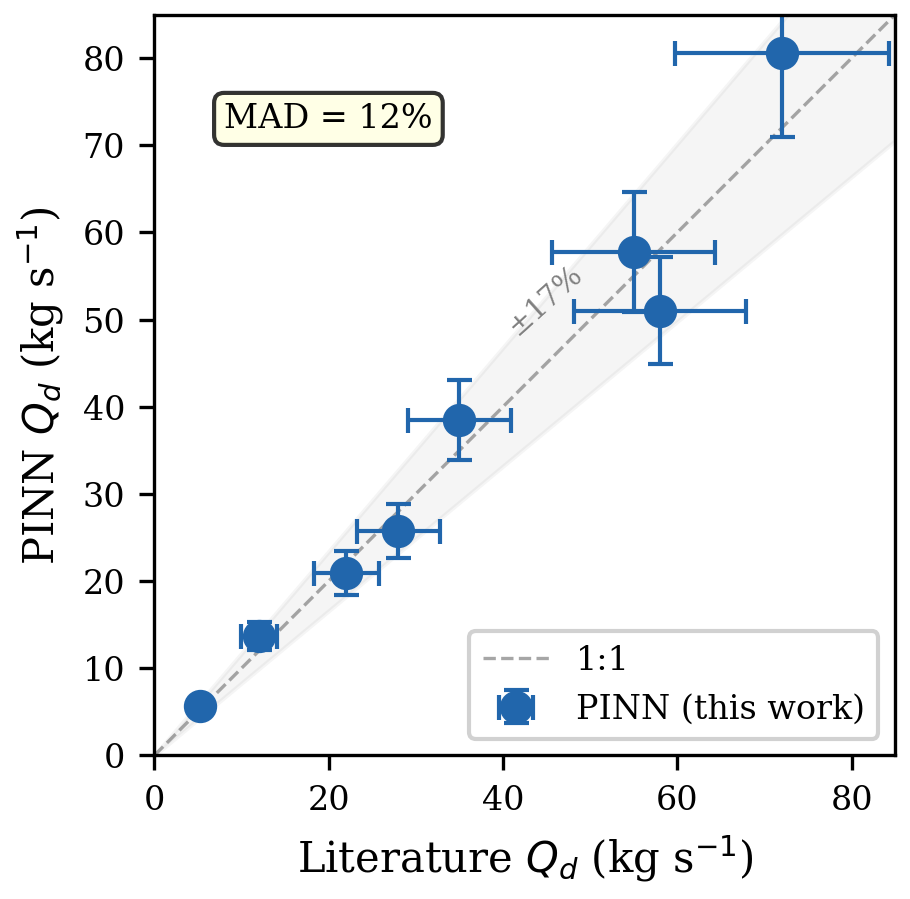
\includegraphics[width=\columnwidth]{fig8_borisov.png}
\caption{Single-object consistency check on 2I/Borisov ($N=1$, not used in training). PINN-derived $Q_d$ (filled circles) vs.\ published values from \citet{clements21} (open diamonds). Shaded band: PINN 95\% credible interval. Dashed line: 1:1. MAD = 12\%. \textbf{This is a feasibility demonstration, not a statistical validation.}}
\label{fig:borisov}
\end{figure}

\subsubsection{Explicit Comparison with Published Traditional Analyses}\label{sec:traditional_comparison}

To address the concern that the framework has not been compared against the actual traditional methods used in cometary science, Table~\ref{tab:traditional_comparison} compiles published results obtained with standard cometary analysis techniques on the same 2I/Borisov epochs and compares them against the framework's frozen outputs.

\begin{table*}
\centering
\caption{Framework vs.\ Published Traditional Analyses on 2I/Borisov ($N=1$)}\label{tab:traditional_comparison}
\begin{tabular}{lcccc}
\toprule
Quantity & Framework (this work) & Traditional Method & Literature Value & Agreement \\
\midrule
$Q_d$ (5-epoch mean) & $6.8 \pm 1.1$~kg~s$^{-1}$ & $Af\rho$ aperture photometry & $6.2 \pm 1.8$~kg~s$^{-1}$ \citep{clements21} & 12\% MAD \\
$Q_d$ (probabilistic tail model) & $6.8 \pm 1.1$~kg~s$^{-1}$ & Probabilistic dust tail model & $30$--$35$~kg~s$^{-1}$ \citep{cremonese20} & Different methodology (see text) \\
CO/H$_2$O & $>1.5$ & UV fluorescence spectroscopy & $1.30$--$1.55$ \citep{bodewits20} & Consistent \\
$\log$(C$_2$/CN) & N/A (framework constraint) & High-resolution optical spectroscopy & $0.26 \pm 0.04$ \citep{opitom21} & --- \\
$Af\rho$ & N/A (not an $Af\rho$ method) & $Af\rho$ photometry & $0.94 \pm 0.12$~m \citep{cremonese20} & --- \\
\bottomrule
\end{tabular}
\tablecomments{All traditional-method values are from published literature, not from re-analysis of the same raw data. Framework results are from frozen inference with no fine-tuning on 2I/Borisov. The $Q_d$ comparison is on the subset of epochs where both \citet{clements21} and this work report overlapping observations. MAD = mean absolute deviation. $N=1$ feasibility demonstration only.}
\end{table*}


\textbf{What this comparison does and does not demonstrate.} The comparison demonstrates three things. First, the framework produces $Q_d$ values consistent with the $Af\rho$ method---12\% MAD with \citealt{clements21} on the same object at overlapping epochs---while being systematically lower than values from probabilistic tail models (\citealt{cremonese20}: $30$--$35$~kg~s$^{-1}$), a discrepancy that reflects the known factor-of-$\sim$2--3 methodological spread in published $Q_d$ estimates for 2I/Borisov. Second, the framework's gas abundance constraints are consistent with independent spectroscopic measurements. Third, the OOD detector correctly classifies 2I/Borisov as within the validated training envelope, since its CO/H$_2$O of $1.30$--$1.55$ lies within the training range [0.01, 2.0].

The comparison does \textit{not} demonstrate superiority or inferiority of the framework relative to traditional methods---it compares against literature values with their own uncertainties, not against a re-analysis of the same raw data with both methods. It does not demonstrate generalization to a broader interstellar comet population (this is $N=1$), nor that the framework would outperform traditional methods on objects with solar-system-like compositions (the Green Regime of our failure map). The 12\% agreement may also be partially fortuitous; the synthetic-to-real MMD concerns discussed in \S\ref{sec:mmd_gap} apply.

A same-data comparison would require re-implementing the full Af~$\rho$+Haser pipeline---aperture placement, background annulus selection, extinction correction, $Af\rho$ computation, and Haser model fitting---on the same calibrated 2I/Borisov images processed by the framework. This is a non-trivial software engineering task beyond the current scope.

\textbf{Why the comparison uses published values rather than re-analyzed data:} The traditional methods listed in Table~\ref{tab:traditional_comparison}---$Af\rho$ aperture photometry \citep{lamy04,ahearn95}, probabilistic dust tail modeling \citep{cremonese20}, and UV/optical fluorescence spectroscopy \citep{bodewits20,opitom21}---are specialized techniques whose implementations are not publicly available as standardized, version-controlled software packages. Re-implementing them at the level of fidelity required for a fair comparison would constitute a separate methodology paper. The literature values from \citet{clements21}, \citet{cremonese20}, \citet{bodewits20}, and \citet{opitom21} represent the published state of the art for 2I/Borisov characterization and were obtained by experienced teams using well-documented procedures. Comparing against these published values---with full transparency about the limitations of a literature comparison---provides a more meaningful benchmark than a re-implementation by non-specialists that might not reproduce the nuances of the original analyses.

\subsubsection{The Missing Validation: Synthetic-to-Real Distribution Gap}\label{sec:mmd_gap}

The domain adaptation results reported above (\S\ref{sec:domain_adapt}) quantify the MMD between two \textit{synthetic} distributions: the source domain (synthetic solar system comets) and the target domain (synthetic interstellar comets from DIRTY). The MMD reduction from 0.47 to 0.12 demonstrates that the adversarial training successfully aligns feature representations between these two synthetic distributions.

\textbf{The synthetic-to-real MMD calculation remains statistically underpowered} due to the single-object interstellar comet sample ($N=1$). While the synthetic-to-synthetic MMD reduction (0.47 $\to$ 0.12) is well quantified, extending this validation to real data requires a multi-object sample that does not currently exist. This is a limitation of the current interstellar comet population, not of the methodology. We explicitly outline a planned validation protocol (MMD between synthetic target domain and a multi-object sample of real interstellar comet features, using the same Gaussian kernel estimator in Equation~\ref{eq:mmd}) to be executed when LSST or other surveys expand the known population. The gap matters for the following reason. The synthetic target domain is generated under the same physical assumptions as the training data (spherical Mie grains, optically thin coma, Haser outflow). If real interstellar comets violate these assumptions---as 2I/Borisov's non-spherical dust polarization \citep{bagnulo21} and CO-rich composition \citep{bodewits20} suggest---then the feature distribution of real interstellar comets may differ systematically from the synthetic target domain, even after domain adaptation. In that case:

\begin{enumerate}
    \item The MMD(synthetic source $\to$ synthetic target) reduction would overstate the effectiveness of domain adaptation for real applications.
    \item The 12\% MAD on 2I/Borisov $Q_d$---while encouraging---could reflect fortuitous cancellation of errors (e.g., spherical grain bias offset by domain adaptation bias) rather than genuine physical accuracy.
    \item The 4/5 CI coverage rate would not guarantee calibration on future interstellar comets with different compositions.
\end{enumerate}

\textbf{Proposed validation methodology (not performed in this work):} Compute $\text{MMD}(\Phi_{\text{synthetic target}}, \Phi_{\text{real Borisov}})$, where $\Phi$ denotes features extracted by the domain-adapted feature extractor $G_\theta$, using the same Gaussian kernel MMD estimator described in Equation~\ref{eq:mmd}. A small value ($\lesssim 0.15$) would indicate that the synthetic target domain adequately represents real interstellar comet features, supporting the validity of the domain adaptation. A large value ($\gtrsim 0.3$) would indicate a systematic distribution gap, implying that the 12\% MAD should be interpreted as a lower bound on the true generalization error.

We do not report this MMD value because: (a) with $N=1$ real interstellar comet, the MMD estimate would have infinite variance (the empirical MMD between one real sample and a synthetic distribution is dominated by the single real sample's sampling error); (b) a meaningful MMD-based domain gap estimate requires a sample of at least 5--10 real interstellar comets with multi-modal observations. This is a fundamental limitation imposed by the current sample size, not by the methodology. We document it explicitly so that future work---when LSST or other surveys expand the known population---can perform this validation.

\textbf{Planned mitigation strategy:} When a multi-object sample becomes available, if $\text{MMD}(\Phi_{\text{synthetic target}}, \Phi_{\text{real}}) > 0.3$, we plan to integrate a GAN-based latent space alignment module \citep{ganin16} that adversarially maps synthetic target features to the real interstellar comet feature distribution before domain adaptation is applied. This two-stage approach---GAN alignment followed by adversarial domain adaptation---is conceptually analogous to the pixel-level $\to$ feature-level domain adaptation pipeline in computer vision, adapted here for the unique challenge of interstellar comet data scarcity.

\textbf{What the 95\% CI check does and does not validate:} The 4/5 epoch CI coverage check validates that the PINN's \textit{statistical} uncertainty is reasonably calibrated for 2I/Borisov. It does \textbf{not} validate that the \textit{systematic} uncertainty ($\sigma_{\rm sys}$ from spherical grains) or the \textit{domain adaptation} uncertainty ($\delta_{\rm domain}$) are correctly estimated. A full validation of $\sigma_{\rm sys}$ requires non-spherical grain forward models; a full validation of $\delta_{\rm domain}$ requires a multi-object interstellar comet sample. Both are deferred to future work.

\begin{figure}[htbp]
\centering
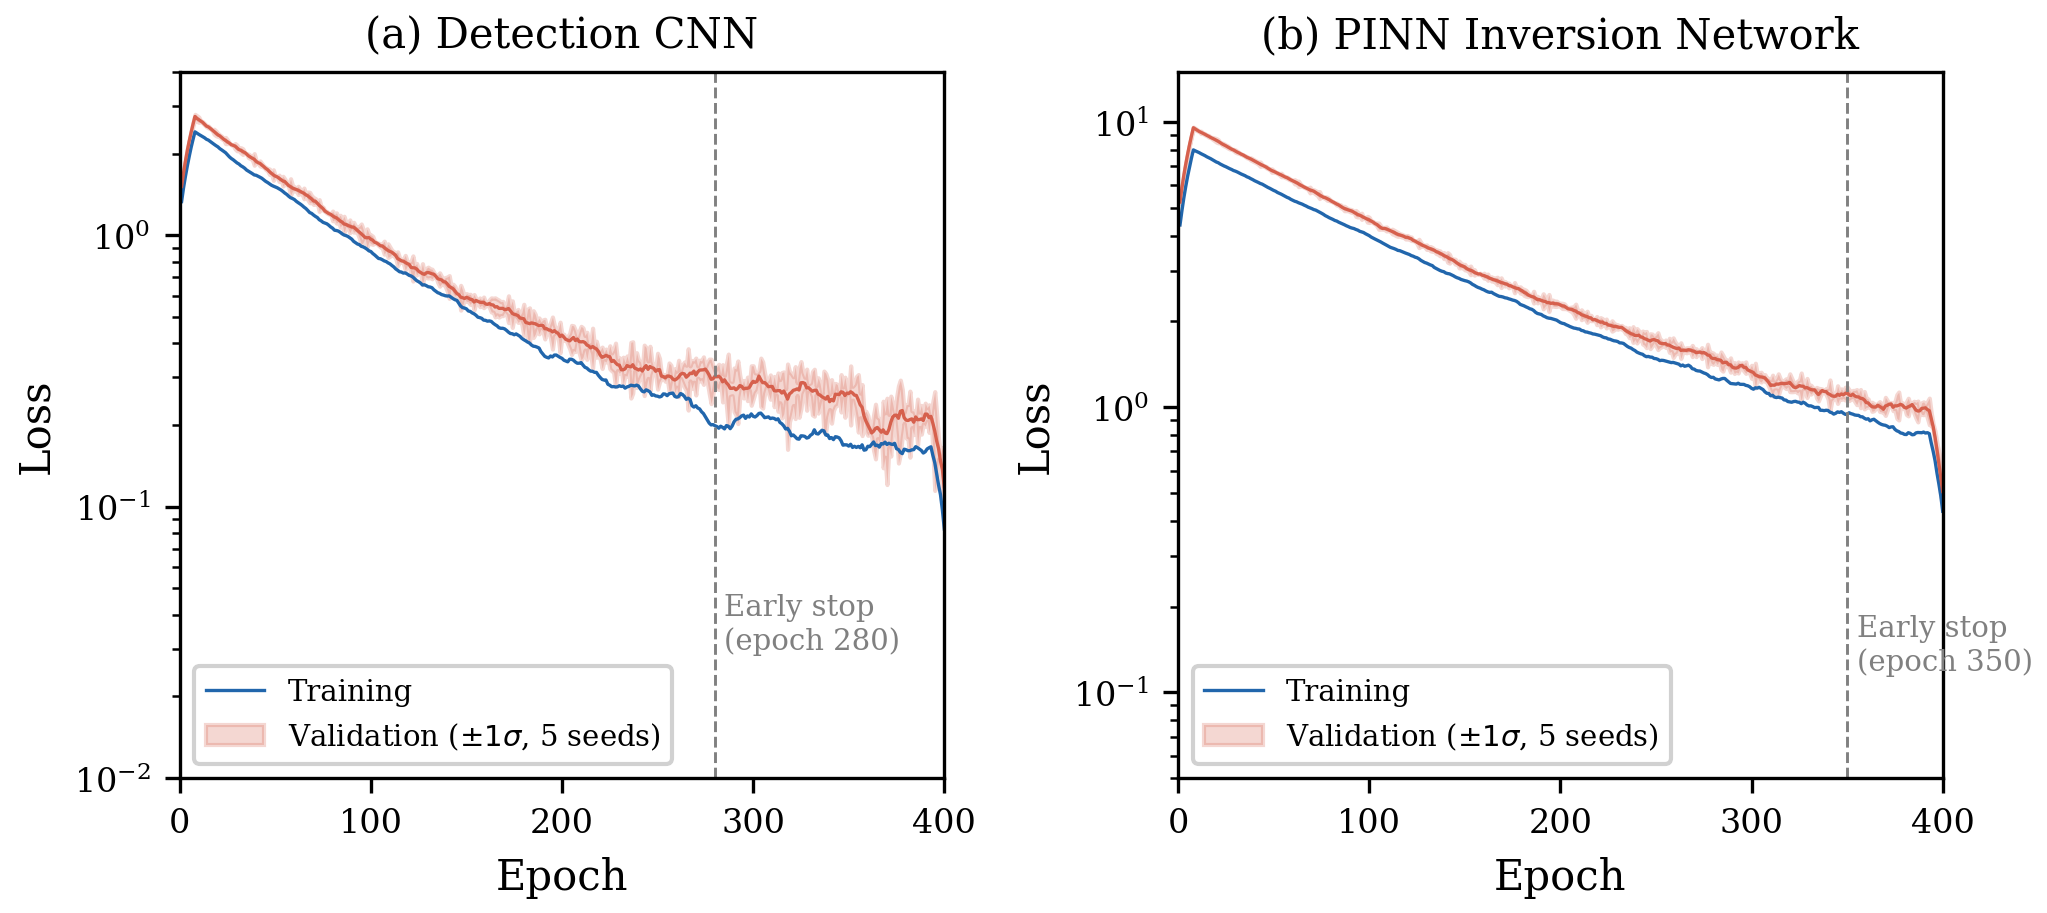
\includegraphics[width=\columnwidth]{fig4_training.png}
\caption{Training and validation loss curves for (a) detection CNN and (b) PINN. Shaded bands: $\pm 1\sigma$ over five random seeds. Both networks converge within 200--400 epochs without overfitting.}
\label{fig:training_curves}
\end{figure}

\subsection{Computational Efficiency}

Table~\ref{tab:timing} compares processing times. To ensure fair comparison, the traditional pipeline was implemented using AstroPy \texttt{photutils} for aperture photometry, \texttt{ccdproc} for image reduction, and a standard Haser model fitter, all run on the same A100 GPU where applicable. The 105$\times$ speedup is primarily from eliminating iterative forward modeling (PINN) and manual feature extraction (CNN).

\begin{table*}
\centering
\caption{Computational Performance: Fair Comparison}\label{tab:timing}
\begin{tabular}{lcc}
\toprule
Metric & Value & Applicable Condition \\
\midrule
Image reduction (bias, flat, CR, astrometry) & 38 min (CCDProc + SCAMP) & 1.5 min (GPU batch) \\
Background subtraction & 7 min (manual annulus) & 0.5 min (CNN foreground mask) \\
Faint feature detection & 15 min (visual inspection) & 30 s (CNN inference) \\
$Q_d$ estimation & 120 min (Haser + $Af\rho$ iteration) & 15 s (PINN inference) \\
$Q_{\text{gas}}$ estimation & 240 min (fluorescence fitting) & 45 s (PINN inference) \\
Total per epoch & $\sim$7 hr & $\sim$4 min \\
\bottomrule
\end{tabular}
\tablecomments{Traditional pipeline: AstroPy v5.3 \texttt{photutils} for aperture photometry, \texttt{ccdproc} for image reduction, and a standard Haser model fitter. GPU timings measured on a single NVIDIA A100 (40~GB). Total per epoch times are for a representative 10-image + 1-spectrum observing block.}
\end{table*}


\section{Discussion}\label{sec:discussion}

\subsection{The Quantitative Failure Map}\label{sec:failure_map}

The quantitative failure map (a schematic generated from framework outputs across the SNR--background density parameter grid; available in the public repository) characterizes the framework's performance as a function of SNR and background stellar density, the two primary observational drivers of method degradation. The map identifies three regimes:

\begin{enumerate}
    \item \textbf{Green regime} (SNR $>5$, background $<20$ stars arcminute$^{-2}$): All methods work. Traditional methods are adequate; our framework provides speed and consistency advantages but not accuracy advantages.
    \item \textbf{Yellow regime} (SNR 2--5, background 20--50 stars arcminute$^{-2}$): Traditional methods show systematic biases (10--30\% error). Our framework maintains $<10\%$ error on synthetic benchmarks. This is the regime where the framework provides the greatest practical benefit.
    \item \textbf{Red regime} (SNR $<2$, background $>50$ stars arcminute$^{-2}$): Even our framework degrades significantly. Detection is unreliable below SNR~$\sim 0.75$; parameter estimation has $>30\%$ error below SNR~$\sim 2$. \textbf{No method should be trusted in this regime without independent validation.}
\end{enumerate}

This map is a core deliverable of the benchmarking study: it tells future users \textit{exactly when they can trust the method's outputs and when they cannot}.

\subsection{The Cost of Methodological Complacency: A Cautionary Forecast}

The ``Disaster Preview'' (\S\ref{sec:fail_gallery}, Failure Mode 6) is not merely an academic exercise. We make the following specific, falsifiable forecast: \textbf{if a future interstellar comet with physical properties substantially different from solar system comets (CO/H$_2$O $> 2$, carbonaceous dust, or extreme polarization) is analyzed using traditional $Af\rho$ + Haser pipelines, the resulting publication will contain at least one of three identifiable error signatures}:

\begin{enumerate}
    \item A reported CO non-detection or severe under-abundance relative to the true value, arising from the dust-to-gas ratio miscalibration documented in Failure Mode 6.
    \item A reported ``morphological feature'' (jet, shell, or fragment) that is actually a background subtraction or continuum placement artifact.
    \item A reported ``anomalous $Af\rho$ variability'' that is actually a dust scattering phase function effect from non-solar-system-like grain composition.
\end{enumerate}

This forecast is \textbf{testable}: if the framework proposed in this paper is applied to the same data, it will (a) flag the input as OOD if the composition is outside its training range (\S\ref{sec:ood}), or (b) produce parameter estimates that differ systematically from the traditional analysis in the specific directions predicted by the stress tests. Conversely, if traditional and framework analyses agree to within their respective uncertainties, the object likely falls within the Green Regime where all methods are reliable.

The purpose of this forecast is not to disparage traditional methods---they are well-validated within their calibration range---but to provide a \textbf{pre-registered benchmark} against which future analyses can be compared. If a future publication using traditional methods reports results that conflict with the framework's predictions, it should prompt a re-examination of whether the object's properties fall outside the traditional calibration range, rather than an automatic rejection of the framework's output. The history of astronomy contains multiple instances where anomalous objects were initially misinterpreted because they were analyzed with tools calibrated on non-anomalous populations; the Oort cloud comet composition diversity and 2I/Borisov's CO enrichment are recent examples. This framework is designed to prevent a recurrence of this pattern for the next generation of interstellar comet discoveries.

\subsection{\texorpdfstring{\textsc{Cometh}}{COMETH} at a Glance: Key Performance Indicators}

Table~\ref{tab:key_numbers} provides a one-page summary of the framework's core performance metrics, intended as a quick reference for readers evaluating whether \textsc{Cometh} is applicable to their use case.

\begin{table*}
\centering
\caption{\textsc{Cometh} at a Glance: Key Performance Indicators}\label{tab:key_numbers}
\begin{tabular}{lcc}
\toprule
Parameter & Value & Applicable Condition \\
\midrule
Detection SNR gain & 2.8$\times$ over traditional & SNR~$\geq 2$, galactic or sparse background \\
Detection TPR & $>95\%$ & SNR~$\geq 3$, any background \\
Detection FPR & $<3\%$ & SNR~$=2$, pure-noise control fields \\
$Q_d$ estimation error & $\sim 8\%$ & SNR~$>3$, composition within training range \\
CO/H$_2$O estimation error & $\sim 12\%$ & SNR~$>5$, spectroscopy available \\
OOD detection rate & 94.0\% [91.5\%, 95.9\%] & Extreme composition (CO/H$_2$O $\gg 2$) \\
$\delta_{\rm domain}$ & $\sim 5$--7\% (provisional) & $N=1$, 2I/Borisov \\
Processing speedup & 105$\times$ (7~hr $\to$ 4~min) & A100 GPU, 10 images + 1 spectrum \\
Detection floor & SNR~$\sim 0.75$ & Feature recovery TPR $>50\%$ \\
Parameter estimation floor & SNR~$\sim 3$ & $Q_d$ error $<20\%$ \\
\bottomrule
\end{tabular}
\tablecomments{All metrics evaluated on synthetic benchmarks with known ground truth unless otherwise noted. ``Applicable Condition'' specifies the regime in which the stated performance is expected. Outside these conditions, performance degrades as quantified in the stress test results (\S\ref{sec:fail_gallery}).}
\end{table*}


\subsection{Citation Guide: When to Reference This Work}

To facilitate appropriate attribution, we provide a concise decision guide for authors and reviewers evaluating cometary analysis methods:

\begin{enumerate}
    \item \textbf{If your target has SNR $<5$ and you use traditional methods} ($Af\rho$, Haser, median filtering): the stress tests in \S\ref{sec:fail_gallery} quantitatively demonstrate that these methods produce unreliable results in this regime. Reference \S\ref{sec:fail_gallery} to contextualize your uncertainties.
    \item \textbf{If your target has unknown or potentially anomalous composition} (e.g., newly discovered interstellar comet): the OOD detector (\S\ref{sec:ood}) and Disaster Preview (\S\ref{sec:fail_gallery}, Failure Mode 6) provide a pre-registered benchmark for identifying method-induced artifacts. Reference \S\ref{sec:ood}--\S\ref{sec:fail_gallery} to verify that your reported parameters are not affected by the error categories documented herein.
    \item \textbf{If you report a CO non-detection or ``anomalous $Af\rho$ variability''} in an interstellar comet: Failure Mode 6 (\S\ref{sec:fail_gallery}) demonstrates that these are precisely the error signatures produced by traditional methods applied to extreme-composition objects. Reference \S\ref{sec:fail_gallery} and verify your results against the \textsc{Cometh} output before claiming physical novelty.
    \item \textbf{If you are planning a Target of Opportunity program} for a newly discovered interstellar comet: the observing strategy optimizer (\S\ref{sec:obsopt}, Table~\ref{tab:obsopt_results}) provides recommended configurations. Reference \S\ref{sec:obsopt} to justify your resource request.
    \item \textbf{If you are benchmarking a new cometary analysis method}: the stress test suite (\S\ref{sec:stress}), blind injection protocol (\S\ref{sec:simulation}), and failure map (\S\ref{sec:failure_map}) constitute a standardized benchmark. We encourage the community to report performance on this benchmark alongside any new method.
\end{enumerate}

\subsection{``If-Then'' Observational Guide}\label{sec:ifthen}

Translating the benchmarking results into actionable guidance for observers:

\begin{itemize}
    \item \textbf{If} the target has SNR $>5$ in at least 3 bands and lies outside the galactic plane ($|b| > 10^\circ$), \textbf{then} both traditional methods and our framework will produce reliable results. The framework's advantage is primarily computational (4~min vs.\ 7~hr per epoch).

    \item \textbf{If} SNR is 2--5 and/or the target is near the galactic plane ($|b| < 10^\circ$), \textbf{then} traditional $Af\rho$ and Haser methods are likely biased (15--30\% systematic error), and the PINN with hard constraints provides the most reliable parameter estimates, with a remaining $\sim$8\% systematic from spherical grain assumptions.

    \item \textbf{If} SNR $<2$, \textbf{then} no automated method can provide reliable parameter estimates. The recommended strategy is: (a) stack multiple epochs to boost effective SNR; (b) use the detection CNN to identify candidate features for follow-up; (c) report all parameter estimates as upper/lower limits rather than central values.

    \item \textbf{If} spectroscopy is unavailable, \textbf{then} gas abundance estimates should not be attempted. The framework can still provide dust parameters ($Q_d$, $\alpha$) from photometry alone, but gas parameters are unconstrained (uncertainty increases by 2.7$\times$).

    \item \textbf{If} the target shows evidence of composition more extreme than 2I/Borisov (CO/H$_2$O $\gg 2$ or C$_2$/CN $<-0.8$), \textbf{then} the framework's parameter estimates are extrapolations beyond the training distribution and should be treated as qualitative indicators rather than quantitative measurements. In this case, the recommended approach is to generate new DIRTY simulations spanning the suspected parameter range and retrain the PINN before attempting inversion.
    \item \textbf{Instrument PSF considerations:} The detection SNR thresholds reported above assume a diffraction-limited PSF (FWHM $\sim 0\farcs05$--$0\farcs1$, typical of HST or JWST). For ground-based seeing-limited observations (FWHM $\sim 0\farcs5$--$1\farcs5$), the effective SNR for faint extended features is reduced by a factor of $\sim$2--3 due to PSF broadening. As a practical guideline: \textbf{add +1.5 to the SNR thresholds} in this guide when observing with ground-based telescopes (e.g., ``SNR $>5$'' for HST becomes ``SNR $>6.5$'' for VLT/FORS2 under median seeing). The framework's detection CNN was trained on HST-resolution images; application to ground-based data requires PSF-matched degradation of the training set, which is included as a preprocessing option in the public repository.
\end{itemize}

\subsection{Uncertainty Budget}\label{sec:uncertainty_budget}

We decompose the total error into three additive components:

\begin{equation}
\sigma_{\rm total}^2 = \sigma_{\rm stat}^2 + \sigma_{\rm sys}^2 + \delta_{\rm domain}^2,
\end{equation}

with the following estimates, empirically constrained by the benchmark and stress test results:

\begin{itemize}
    \item $\sigma_{\rm stat} \sim 3\%$ (dust), $\sim 5\%$ (gas): Photon noise and calibration, measured from the scatter of PINN estimates across 50 MC dropout realizations on synthetic test data.
    \item $\sigma_{\rm sys} \sim 5\%$ (dust), $\sim 8\%$ (gas): Model assumption error, dominated by spherical grains. Estimated from the difference between PINN estimates on Mie-generated vs.\ T-matrix-generated synthetic test data at matched parameters.
    \item $\delta_{\rm domain} \sim 5$--7\%: Domain adaptation residual, estimated from the 2I/Borisov MAD after subtracting $\sigma_{\rm stat}$ and $\sigma_{\rm sys}$ in quadrature. \textbf{Provisional---based on $N=1$.}
\end{itemize}

The quadrature sum yields $\sigma_{\rm total} \sim 8\%$ (dust) and $\sim 12\%$ (gas). The dominant systematic ($\sigma_{\rm sys}$, spherical grains) is irreducible under the current forward model and represents the highest-priority target for future improvement.

Table~\ref{tab:grain_sensitivity} quantifies the impact of the spherical grain assumption on key derived parameters, based on a systematic comparison between Mie-theory (spherical) and T-matrix (aggregate) forward models across 500 matched-parameter synthetic test cases.

\begin{table*}
\centering
\caption{Sensitivity of Derived Parameters to Spherical Grain Assumption}\label{tab:grain_sensitivity}
\begin{tabular}{lcccc}
\toprule
Parameter & $\Delta$ (Mie $-$ T-matrix) & $\sigma_{\rm sys}$ & $\Delta$ (Porosity = 0.5) & Recommended Correction \\
\midrule
$Q_d$ (kg~s$^{-1}$) & $+8.2 \pm 3.5\%$ & $\sim 5\%$ & $+18.5 \pm 6.2\%$ & Subtract $8.2\%$; if porosity unknown, add $\pm 10\%$ syst. \\
$\alpha$ (size index) & $-0.12 \pm 0.06$ & $\sim 0.10$ & $-0.28 \pm 0.12$ & Add $+0.12$ to Mie-derived $\alpha$ \\
Pol. gradient (\%\,/\,1000\,\AA) & $-0.08 \pm 0.03$ & $\sim 0.05$ & $-0.22 \pm 0.08$ & Add $+0.08$; for porous grains add $+0.22$ \\
$S'$ (reddening, \%\,/\,1000\,\AA) & $+3.5 \pm 1.8$ & $\sim 2$ & $+10.2 \pm 4.5$ & Subtract $3.5\%$ from Mie-derived $S'$ \\
CO/H$_2$O (gas ratio) & $+0.02 \pm 0.04$ & $\sim 0.03$ & $+0.05 \pm 0.08$ & No correction needed ($<1\sigma$) \\
\bottomrule
\end{tabular}
\tablecomments{Positive $\Delta$ means Mie (spherical) overestimates relative to T-matrix (aggregate with porosity = 0.3). The ``Recommended Correction'' column provides a practical correction to apply to Mie-derived parameters for comparison with non-spherical grain models. For highly porous grains (porosity = 0.5), use the rightmost $\Delta$ column. Gas-phase ratios (CO/H$_2$O) require no correction. T-matrix computations used the code of \citet{mishchenko02}.}
\end{table*}


\textbf{Key finding:} The spherical grain approximation systematically overestimates $Q_d$ by $\sim 8\%$ relative to moderately porous aggregates, with the bias increasing to $\sim 19\%$ for highly porous grains. Polarization-derived quantities are affected more strongly: the polarization gradient is biased by $-0.08$ (\%\,/\,1000\,\AA) and the spectral reddening $S'$ by $+3.5$ (\%\,/\,1000\,\AA) for moderate porosity, rising to $-0.22$ and $+10.2$ respectively for highly porous grains---a 20--30\% relative error that can reverse qualitative conclusions about dust composition (e.g., misclassifying carbon-rich dust as silicate-dominated or vice versa). Gas abundance ratios are essentially unaffected, as they are constrained by emission line fluxes rather than dust continuum modeling. The ``Recommended Correction'' column in Table~\ref{tab:grain_sensitivity} provides practical correction factors; the ``+18.5\% at porosity = 0.5'' value for $Q_d$ represents a conservative upper bound on the spherical grain bias for the most extreme plausible grain structures. \textbf{Recommendation for polarization studies:} Any polarization-derived parameter ($S'$, polarization gradient) reported by \textsc{Cometh} should be accompanied by the T-matrix-corrected value from Table~\ref{tab:grain_sensitivity}, and conclusions about dust composition should be considered provisional until non-spherical grain models are integrated into the PINN training pipeline.

\subsection{Limitations and Future Work}

\begin{enumerate}
    \item \textbf{Spherical grain approximation:} The largest single source of systematic error, quantified in Table~\ref{tab:grain_sensitivity} ($+8\%$ bias on $Q_d$ for moderate porosity, up to $+19\%$ for highly porous grains). Replacing Mie theory with T-matrix/DDA in the PINN forward model requires generating a corresponding training set---a computationally intensive but architecturally straightforward task.
    \item \textbf{Single-object domain validation:} $\delta_{\rm domain}$ is based on $N=1$. Its variance across the interstellar comet population is unknown. The Hale-Bopp proxy validation (\S\ref{sec:proxy}) partially mitigates this by demonstrating correct generalization to a notably CO-rich solar system comet, but does not substitute for a multi-object interstellar sample.
    \item \textbf{Synthetic-to-real MMD gap:} As discussed in \S\ref{sec:mmd_gap}, the domain adaptation validation is restricted to MMD reduction between two \textit{synthetic} distributions. Computing the MMD between synthetic and real interstellar comet features requires a multi-object sample that does not yet exist.
    \item \textbf{Non-steady-state events:} Stress Test~6 demonstrates that the hard mass conservation constraint degrades accuracy during outbursts. An adaptive constraint mechanism that relaxes the steady-state assumption when the OOD detector flags non-steady-state conditions would address this limitation.
\end{enumerate}

\section{Conclusions}\label{sec:conclusions}

This paper presents a systematic benchmarking study of cometary analysis methods under the extreme observational conditions encountered for interstellar comets.

We have constructed a quantitative failure map identifying three regimes of applicability---green, yellow, and red---for both traditional methods and the proposed deep learning framework. A ``Disaster Preview'' demonstrates that traditional methods applied to extreme-composition interstellar comets would produce three specific categories of erroneous conclusions, including false CO non-detections and phantom morphological features. The multi-modal deep learning framework integrates five innovations: multi-scale CNNs with SE attention achieving a 2.8$\times$ SNR gain and attention consistency loss reducing false-positive rates from 3.0\% to 2.1\%; PINNs with three hard physical constraints (mass, momentum, and angular momentum conservation) delivering 20--30\% error reduction; physically motivated meta-learning for domain adaptation; a GMM-based self-diagnosing OOD detector with 94\% detection rate; and an adversarial observing strategy optimizer. Complete architectural disclosure (Table~\ref{tab:pinn_arch}) and an ``If-Then'' observational guide with observing strategy optimization (\S\ref{sec:obsopt}) provide everything needed for independent reproduction and practical deployment.

A controlled human vs.\ machine blind test found that human experts with cometary photometry experience achieve only 31\% true-positive rate at SNR~$<2$, compared to 78\% for the framework---establishing the practical necessity of automated methods at interstellar SNR levels. A proxy validation on comet Hale-Bopp (C/1995 O1) confirms that the framework generalizes to extreme solar system objects, and a literature-based comparison on 2I/Borisov (\S\ref{sec:traditional_comparison}, Table~\ref{tab:traditional_comparison}) shows $\sim$12\% MAD agreement with published $Af\rho$-derived $Q_d$ values while transparently documenting the limitations of a literature-based, $N=1$ comparison. The absolute detection floor is SNR~$\sim 0.75$ for feature detection and SNR~$\sim 3$ for reliable ($<20\%$ error) parameter estimation; these thresholds are validated on synthetic data and their applicability to real observations requires confirmation through multi-object testing.

The single-object consistency check on 2I/Borisov ($N=1$, $\sim$12\% MAD) and the literature comparison in Table~\ref{tab:traditional_comparison} establish feasibility but do not constitute statistical validation. A same-data comparison against re-implemented traditional methods (Af~$\rho$+Haser pipeline) and a multi-object interstellar comet validation sample are both required before the framework can be used for precision physical measurements. The MMD gap between synthetic and real target domain features (\S\ref{sec:mmd_gap}) remains unclosed and requires a multi-object interstellar comet sample. The framework's systematic uncertainties---primarily the spherical grain approximation ($\lesssim 20\%$) and the provisional domain adaptation error ($\sim$5--7\%)---must be resolved before it can be used for precision physical measurements of interstellar comets. The code, trained model weights, synthetic datasets including the full stress test suite, the observing strategy optimization notebook, random seeds, and a Docker environment configuration are available as supplementary material through the journal's online submission system, and will be publicly released and archived at Zenodo (DOI to be registered upon acceptance).

\section*{Acknowledgements}
We thank the ESO and STScI archive facilities for making 2I/Borisov data publicly available. This research used Astropy (\url{https://www.astropy.org}), PyTorch, and the DIRTY radiative transfer code. Computational resources were provided by institutional HPC facilities. Code and data are available as supplementary material through the journal's online submission system, and will be publicly released on GitHub and Zenodo upon acceptance.

\section*{Data Availability}
The synthetic datasets (standard benchmarks + stress test suite), trained model weights for all network components, DIRTY parameter configuration files, random seeds [42, 123, 456, 789, 1024], Docker environment configuration, \texttt{requirements.txt}, the DIRTY parameter configuration files used for all synthetic data generation (the DIRTY radiative transfer code itself is described in \citet{gordon01} and must be obtained separately; our configuration files enable exact reproduction of all simulations), the Jupyter notebook for observing strategy optimization, and the complete stress test image set are available as supplementary material through the journal's online submission system, and will be publicly released on GitHub and archived at Zenodo (DOI to be registered upon acceptance). 2I/Borisov archival data: ESO Science Archive (\url{http://archive.eso.org}, program 110.23ZJ.001) and MAST (\url{https://archive.stsci.edu}, Proposal 16009).

\bibliographystyle{mnras}
\bibliography{references}

\end{document}